\chapter{Reliability and Standard Residuals} \label{appendices:RedStdResComp}

The geometry and number of observations obtained for a particular survey can heavily impact the final solution, the associated formal uncertainty of that solution, and the ``reliability'' of that solution. The term ``reliability'' refers to the robustness of the survey to significant biases and blunders in the observations.

There are three primary reliability metrics than can be computed for each observation employed in a survey: local reliability, otherwise known as redundancy, derived in section B.1; internal reliability, otherwise known as the minimum detectable bias, derived in section B.2; and external reliability vectors, which are the minimum detectable bias values mapped through the state update equation, derived in section B.3. The magnitude of the external reliability vectors can provide a sense of the relative impact a minimum detectable bias has on the state (e.g. each position that is estimated), and thus the RSS (root-sum-square) magnitude is computed and provided for each observation. The external reliability vectors can be bounded by a ``reliability rectangle'' which provides a visual indication of the impact any lack of reliability in the observations has on the final estimated positions. 

Overall these reliability metrics provide the surveyor a sense of susceptibility in the estimated positions to blunders and outliers in the observations, and thus where they may want/need to strengthen their network of observations by adding more observations and/or improving the geometry of those observations (e.g. adding range measurements in the direction of the rectangle major axis) in order to obtain a sufficiently reliable solution and formal covariance. The reliability metrics can also be part of the final deliverable product to customers,
informing the reliability of the solutions and covariance provided.

In addition to reliability metrics, standard residuals are computed for each observation of a survey adjustment, and are provided in the ``Measurement Residuals'' table within the SALSA UI. This appendix details the derivation and utility of these values when employing SALSA in a survey adjustment.

\section{Redundancy}

The redundancy metric, also known as the ``partial redundancy'' and ``local reliability'' value, indicates how susceptible the solution is to errors in that observation, and thus larger redundancy values are better than small values. If there are observations with very small redundancy values, more observations may be needed (thus increasing the redundancy) to safeguard against blunders or outliers in those observations.

First the relationship between the observations vector $\textbf{Y}$ and the post-fit raw residuals vector $\textbf{R}_{raw}$ is derived:
\begin{equation}\label{eq:vhat}
\begin{split}
\textbf{R}_{raw} &= \textbf{Y} - H \hat{\textbf{x}} \\
&= \textbf{Y} - H \; \text{Cov} \; H^T \; \text{MCov}^{-1} \; \textbf{Y} \\
&= Q_{RR} \; \text{MCov}^{-1} \; \textbf{Y} \\
&= R \; \textbf{Y} \\
\end{split}
\end{equation}
where $H$ is the measurements partials derivatives matrix with respect to the estimated state, $\hat{\textbf{x}}$ is the estimated state, $\text{Cov}$ is the post-fit formal estimated state covariance, $\text{MCov}$ is the prescribed measurement noise covariance matrix, $R$ is the redundancy matrix (the diagonals of which are the redundancy values $r_i$ for each observation), and $Q_{RR}$ is the ``residuals cofactor matrix'':
\begin{equation}\label{eq:Qrr} %\label{eq:ResCov}
Q_{RR} = \text{MCov} - H \: \text{Cov} \: H^T
\end{equation}
$R = Q_{RR} \; \text{MCov}^{-1}$ represents the linear transformation between the observations and the residuals, or the ``proportionality factor'' between gross errors and the residuals. 

Thus the effect on an individual residual $R_{raw,i}$ from an individual blunder $\Delta Y_i$ on observation $i$ is
\begin{equation}\label{eq:BlunderImpactOnRes}
	\begin{split}
		\Delta R_{raw,i} &= \frac{Q_{RR_{ii}}}{\text{MCov}_{ii}} \Delta Y_i \\
		&= r_i \; \Delta Y_i
	\end{split}	
\end{equation}
Thus the vector of individual redundancy values for each observation can be assembled from the diagonal elements of $R$:
\begin{equation}\label{eq:Redundancy}
\begin{split}
\textbf{Rd} &= \left[ r_1 \;\; r_2 \;\; \cdots \right] \\
&= \left[Q_{RR,11} \text{MCov}^{-1}_{11} \;\; Q_{RR,22} \text{MCov}^{-1}_{22} \;\; \cdots \right]
\end{split}
\end{equation}
where $Q_{RR,ii}$ is the $i^{\text{th}}$ diagonal element of $Q_{RR}$, and $\text{MCov}^{-1}_{ii}$ is the $i^{\text{th}}$ diagonal element of inverted measurement noise covariance $\text{MCov}^{-1}$.

The redundancy value $r_i$ varies from 0 to 1:
\begin{itemize}
	\item A redundancy of 0 indicates no redundancy at all in the observation, and thus there is no impact on the residual (which remains zero). Any error in the observation goes straight into the state, and thus it is impossible to identify any blunders.
	\item A redundancy of 1 indicates perfect redundancy that is achievable only with infinite observations, thus a value of 1 is never actually achieved, but rather approached as the number of redundant measurements increases. Any error in the observation is almost perfectly reflected in the residual, almost none of the error will go into the solution, and thus it is trivial to identify the blunder.
\end{itemize}

Note how in equation \ref{eq:Qrr} the post-fit formal state covariance $\text{Cov}$ is mapped into the measurement space via $H$. If any of the states map 1-to-1 into the measurement space (i.e. there is only measurement for a particular state), mapping the state covariance value into measurement space via $H$ produces a covariance value for that observation that is equal to the measurement noise covariance value for that observation, and thus the difference value when computing $Q_{RR}$ is zero (i.e. the redundancy is zero). As the number of observations associated with a particular state increases, the magnitude of the associated post-fit formal state uncertainty drops, the resulting mapped covariance for those observations drops, the associated values in $Q_{RR}$ approach the associated measurement noise covariance matrix $\text{MCov}$, and thus the associated redundancy values in $R = Q_{RR} \; \text{MCov}^{-1}$ approach 1. 

Also note how the redundancy values are not at all dependent on the actual observation values: only the structure of the survey adjustment (i.e. the geometry, types, and number of observations obtained) affects the redundancy values.  Thus surveyors can employ SALSA to ensure all observations have reasonable redundancy when designing the structure of the survey. Ghilani \cite{ghilani} states ``The redundancy numbers provide insight into the geometric strength of the adjustment.'' He also states ``Redundancy numbers above 0.5 are generally sufficient to provide well-checked observations.''

The sum of the redundancy values for all observations, i.e. the trace of $R$ or the sum of $\textbf{Rd}$, is equal to the degrees of freedom $N_{DOF}$ of the estimation problem:
\begin{equation}\label{eq:SumRed}
\sum_i r_i = N_{DOF} = N_{obs} - N_{unknowns}
\end{equation}
where $N_{obs}$ is the total number of observations and $N_{unknowns}$ is the number of estimated states. Thus $N_{DOF}$ can be thought of as the overall redundancy of the survey adjustment, and an individual redundancy value is the share of that overall redundancy attributed to the corresponding individual observation. 

\section{Standard Residuals} \label{sect:StdRes}

The standard residual is a metric often used to identify and correct potentially erroneous, unreasonable, or problematic measurements (e.g. from user blunders during the survey, or outliers resulting from unmodeled forces with large tails). Also known as ``standardized'' residuals, or ``studentized'' residuals, standard residual values are computed for every observation in SALSA adjustments. The process of reviewing the standard residuals and removing or correcting any problematic observations is often called ``data snooping'' in the literature.

\subsection{Supporting quantities}

To compute the standard residual value for an observation, several other quantities are first needed. First the relative residual vector is computed:
\begin{equation}\label{eq:RelRes}
\textbf{R}_{rel} = \sqrt[c]{\text{MCov}}^{-1} \textbf{R}_{raw} \;\; \left( \sqrt[c]{\text{MCov}} \sqrt[c]{\text{MCov}}^T = \text{MCov} \right)
\end{equation}
where $\sqrt[c]{\text{MCov}}$ is the Cholesky decomposition \cite{golub1996matrix} of the measurement noise covariance matrix $\text{MCov}$.

Next the Chi-Squared metric \cite{ghilani} is computed for the entire adjustment:
\begin{equation}\label{eq:ChiSquared}
\chi^2 = \left( \text{RMS}\left(\textbf{R}_{rel}\right)\right)^2 N_{obs}
\end{equation}
where $\text{RMS}\left(\textbf{R}_{rel}\right)$ is the root-mean-square of the relative residual vector $\textbf{R}_{rel}$. 

The a posteriori variance of unit weight (APV) is easily computed from the Chi-Squared metric:
\begin{equation}\label{eq:APV}
\text{APV} = \chi^2 / N_{DOF}
\end{equation}

\subsection{Standard residual derivation}

A standard residual value is actually a test metric computed for a hypothesis test:
\begin{equation}\label{eq:HypTest}
\begin{split}
H_0 : \;\; &E[\Delta Y_i] = 0 \\
H_A : \;\; &E[\Delta Y_i] \ne 0
\end{split}
\end{equation}
where $\Delta Y_i$ is a potential blunder on observation $i$, $H_0$ is the hypothesis that observation $i$ is not an outlier, and $H_A$ is the hypothesis that observation $i$ is an outlier.

The test metric is a standard z-test metric, dividing the potential blunder $\Delta Y_i$ by the uncertainty of that potential blunder:
\begin{equation}\label{eq:TestMetric}
T_X = \frac{\Delta Y_i}{\sigma_{\Delta Y_i}}
\end{equation}

The uncertainty value $\sigma_{\Delta Y_i}$ is computed as
\begin{equation}\label{eq:SigmaY}
\begin{split}
\sigma_{\Delta Y_i}^2 &= \left( \frac{\partial Y_i}{\partial R_{raw,i}} \right)^2 \sigma_{\textbf{R}_{raw}}^2 \\
&= \left( \frac{\text{MCov}_{ii}}{Q_{RR,ii}}\right)^2 \left(\text{APV} \; Q_{RR,ii}\right) \\
&= \text{APV} \; \frac{\text{MCov}_{ii}^2}{Q_{RR,ii}} \\
\sigma_{\Delta Y_i} &= \sqrt{\text{APV}} \; \frac{\text{MCov}_{ii}}{\sqrt{Q_{RR,ii}}}
\end{split}
\end{equation}
where the raw residual variance $\sigma_{\textbf{R}_{raw}}^2 = \text{APV} \; Q_{RR,ii}$, and the partial derivative $\frac{\partial Y_i}{\partial R_{raw,i}}$ is obtained from equation \ref{eq:BlunderImpactOnRes}.

The test metric $T_X$ (i.e. standard residual) is then computed:
\begin{equation}\label{eq:TestMetricStdRes}
\begin{split}
T_X &= \frac{\Delta Y_i}{\sigma_{\Delta Y_i}} = \frac{\text{MCov}_{ii}}{Q_{RR,ii}} R_{raw,i} \frac{\sqrt{Q_{RR,ii}}}{\sqrt{\text{APV}} \; \text{MCov}_{ii}} \\
&= \frac{R_{raw,i}}{\sqrt{\text{APV} \; Q_{RR,ii}}} = \frac{R_{raw,i} / \sqrt{\text{MCov}_{ii}} }{\sqrt{\text{APV} \; Q_{RR,ii} / \text{MCov}_{ii}}} = \frac{R_{rel,i}}{\sqrt{\text{APV} \; r_i}}
\end{split}
\end{equation}

The standard residuals for all observations, collected into a vector, is
\begin{equation}\label{eq:StdResVect}
\textbf{R}_{std} = \left[ R_{rel,1} / \sqrt{\text{APV} \cdot r_1} \;\;\; R_{rel,2} / \sqrt{\text{APV} \cdot r_2} \;\;\; \cdots \right]
\end{equation}

Thus the standard residual is a further ``normalization'' of the relative residual involving the APV and the redundancy of the measurement. Note that having the redundancy value in the denominator of each standard residual value means that if the redundancy is very small, the standard residual may be especially high and thus less reliable as a blunder test (described in more detail below). If a measurement's redundancy is zero (undesirable for any measurement in any survey), the associated standard residual is infinite (and thus not computable).

\subsection{Standard residual test threshold}

After computing the standard residual value, the value is compared to a threshold based on a user-provided confidence value and assumed probability density function (PDF) in order to ascertain whether the hypothesis test passes or fails. A visualization of this threshold is provided via the ``accepted'' and ``rejected'' regions in figure \ref{Fig:HypTest}, along with the PDF $f_X$, standard residual test metric $T_X$, and significance level $\alpha$ that defines the threshold.
\begin{figure} [!htb]
	\centering
	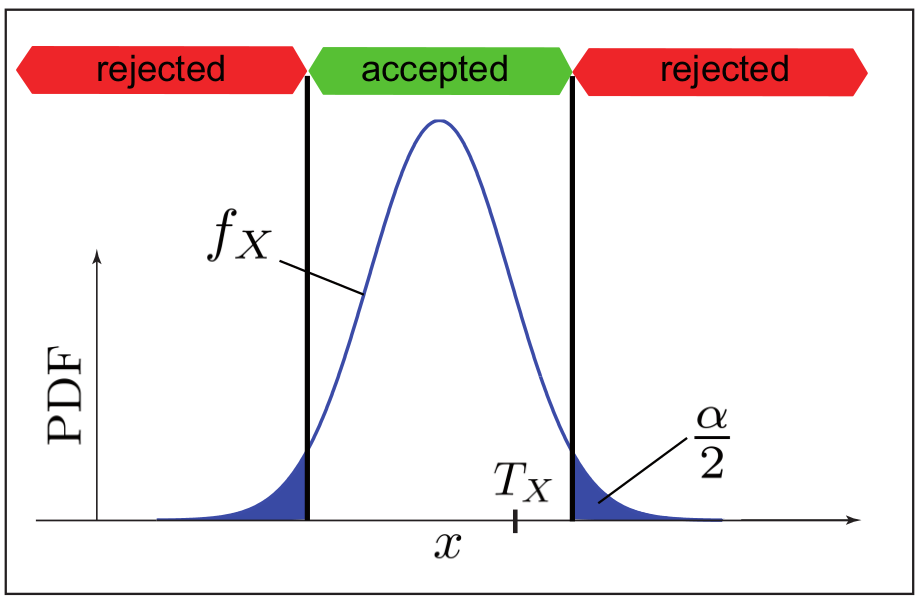
\includegraphics[trim = 0mm 0mm 0mm 2mm, clip, width=0.6\textwidth]{figures/SebastianNotesScreenshots/Screenshot2020-02-21t15-00-11.png}
	\caption{Hypothesis test}
	\label{Fig:HypTest}
\end{figure}

The significance level $\alpha = 1 - \text{Confidence}$, where $\text{Confidence}$ is the confidence value provided by the user, is typically equal to 0.95 or 0.99 (95\% or 99\%). For example, if the user specifies a 99\% confidence level, $\alpha = 0.01$. 

The most common PDF employed in a standard hypothesis test is the classic Gaussian (i.e. normal) distribution, for which regions of acceptance (i.e. $H_0$ is declared true) are:
\begin{itemize}
	\item $\approx \pm 1.96$ for $\alpha = 0.05$ (95\% confidence)
	\item $\approx \pm 2.58$ for $\alpha = 0.01$ (99\% confidence)
	\item $\approx \pm 3.29$ for $\alpha = 0.001$ (99.9\% confidence)
\end{itemize}
Ghilani \cite{ghilani} states ``In practice, authors have reported that a value of 3.29 also works as a criterion for rejection of blunders.'' 

However, the use of the Gaussian distribution is applicable only when the possible values for the standard residuals can extend infinitely in the positive or negative direction. When the a priori variance of unit weight, which describes how the least squares weighting matrix and the inverse of the measurement noise covariance are related (and thus is typically equal to identity), is used in lieu of the APV in equations \ref{eq:TestMetricStdRes} and \ref{eq:StdResVect}, as described in Ghilani \cite{ghilani} and Leick \cite{leick}, the assumption of infinite tails for the standard residual is reasonable. But when the APV is used as described in equations \ref{eq:TestMetricStdRes} and \ref{eq:StdResVect}, a different distribution is needed: the tau distribution, as described in section \ref{sec:TauDist}.

\subsection{Tau distribution} \label{sec:TauDist}

Unlike the standard residual formulations provided in Ghilani \cite{ghilani} and Leick \cite{leick}, a different convention is employed in Vanicek \& Krakiwsky (Chapter 13) \cite{vanicek1982geodesy} and Deakin \cite{deakin2018tau}: the APV is employed in the standard residual, as described in equations \ref{eq:TestMetricStdRes} and \ref{eq:StdResVect}. As a result of employing the APV, the standard residuals have finite limits. To derive these limits, first the standard residual is reformatted:
\begin{equation}\label{eq:StdRes}
\begin{split}
R_{std,i} &= \frac{R_{rel,i}}{\sqrt{\text{APV} \cdot r_i}} \\
&= \frac{R_{rel,i}}{\sqrt{\frac{(\text{RMS}(\textbf{R}_{rel}))^2 N_{\text{obs}}}{N_{\text{DOF}}} \; r_i}} \\
&= \frac{R_{rel,i}}{\sqrt{\frac{(\sum_{j=1}^{m} R_{rel,j}^2/N_{\text{obs}}) N_{\text{obs}}}{N_{\text{DOF}}} \; r_i}} \\
&= \frac{R_{rel,i}}{\sqrt{\sum_{j=1}^{m} R_{rel,j}^2}} \frac{\sqrt{N_{\text{DOF}}}}{\sqrt{r_i}}
\end{split}
\end{equation}
As a particular relative residual $R_{rel,i}$ approaches infinity, the finite limit of the standard residual is revealed:
\begin{equation}\label{eq:StdResLimit}
R_{std,i} \rightarrow \pm \frac{\sqrt{N_{\text{DOF}}}}{\sqrt{r_i}} \;\; \text{as} \;\; R_{rel,i} \rightarrow \pm \infty
\end{equation}

Note that the standard residual formulation in equations \ref{eq:TestMetricStdRes} and \ref{eq:StdResVect} is also referred to as an ``internally studentized residual''. In this formulation, the APV value is computed using all post-fit observation residuals, including any potential outliers. Because any anomalous residuals are included in the computation of the APV, which is in turn used to ``studentize'' or ``standardize'' the residuals, as a particular observation residual approaches infinity, the corresponding standard residual approaches the finite limit shown in equation \ref{eq:StdResLimit}. An alternative formulation is the ``externally studentized residual'', in which the APV does \textbf{not} include potential outliers. This formulation can have infinite limits as a result, but is not widely used.

When a scenario has non-infinite DOF, which is true for any adjustment performed in SALSA, alternatives to the Gaussian distribution are more representative of the relevant PDFs. One commonly used alternative is Student's t-distribution. However, the t-distribution has infinite tails, unlike the standard residual formulation in equations \ref{eq:TestMetricStdRes} and \ref{eq:StdResVect}. Thus a different alternative is employed: the tau distribution, as described in Pope \cite{pope1976statistics}, and Thompson \cite{thompson1935criterion}, and as illustrated in figure \ref{Fig:TauDist}.
\begin{figure} [!htb]
	\centering
	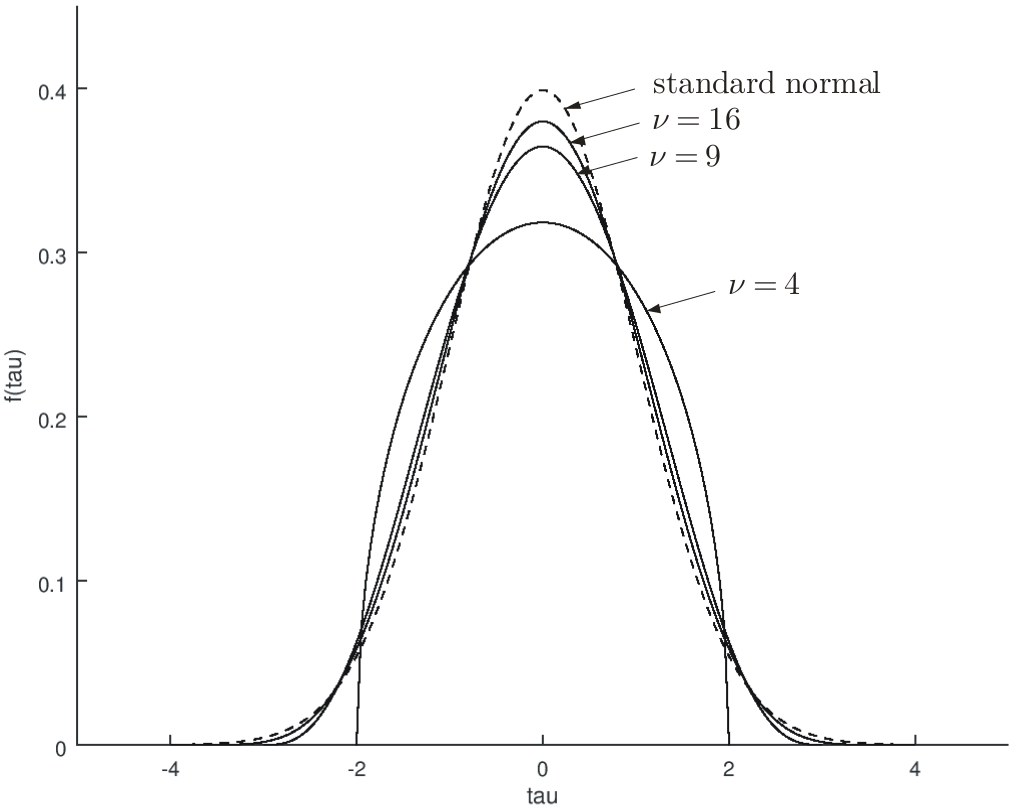
\includegraphics[trim = 0mm 0mm 0mm 0mm, clip, width=0.63\textwidth]{figures/DeakinScreenshots/TauDistributionCurves.png}
	% TwoSidedTest.png
	% Trim option parameter order: left bottom right top
	\caption{Tau distribution for different DOF ($\nu$)}
	\label{Fig:TauDist}
\end{figure}

Note how in figure \ref{Fig:TauDist} the tau distribution with DOF $\nu = 4$ has finite limits of $\pm 2$, and as the number of DOF increases, the tau distribution approaches the normal distribution (like the t-distribution). 

The tau distribution is closely tied to the t-distribution:
\begin{equation}\label{eq:TauEqn}
\tau_{\nu} = \frac{t_{\nu-1} \sqrt{\nu}}{\sqrt{\nu - 1 + t_{\nu-1}^2}}
\end{equation}
where $t_{\nu-1}$ is the t-distribution with $\nu - 1$ DOF.

If the value of $t$ within equation \ref{eq:TauEqn} approaches infinity, the finite limit of the tau distribution is revealed (suppressing subscripts):
\begin{equation}\label{eq:TauLimits}
\lim_{t \to \pm\infty} \tau = \lim_{t \to \pm\infty} \frac{t \sqrt{\nu}}{\sqrt{\nu - 1 + t^2}} = \sqrt{\nu} \lim_{t \to \pm\infty} \frac{t}{\sqrt{\nu - 1 + t^2}} = \pm \sqrt{\nu}
\end{equation}

To summarize, because the standard residual formulation provided in equations \ref{eq:TestMetricStdRes} and \ref{eq:StdResVect} has non-infinite limits, the tau distribution is the most appropriate distribution to use when computing thresholds for hypothesis testing: if the probability of standard residual values beyond those finite limits is zero, the PDF employed should reflect that reality. This reality also implies that if the a priori variance of unit weight (typically identity) is employed rather than the APV when computing standard residuals, a distribution with infinite tails such as the normal or t-distribution is more appropriate. 

Readers may note that the finite limits in equations \ref{eq:StdResLimit} and \ref{eq:TauLimits} are not identical: the standard residuals are bounded by $\pm \frac{\sqrt{\nu}}{\sqrt{r_i}}$, while the tau distribution is bounded by $\pm \sqrt{\nu}$. Section \ref{sec:ComputeThreshold} details how the tau distribution is scaled by $\frac{1}{\sqrt{r_i}}$ to appropriately account for the finite limits of the standard residuals. 

\subsection{Computing Threshold Values For Tau Distribution} \label{sec:ComputeThreshold}

To compute the hypothesis test threshold value using the tau distribution, first a confidence interval value must be specified. The value employed within SALSA is 95\%, or 0.95, which corresponds to a significance level $\alpha = 0.05$. If a larger confidence value is employed, the threshold values become larger, and thus fewer standard residuals will fail the statistical test.

SALSA employs a ``two-sided'' hypothesis test: the 5\% rejection region includes the area under the PDF curve for both sides of the distribution, as depicted in figure \ref{Fig:HypTest}. Because the tau distribution is symmetric, the area under the PDF curve for the right-side tail is $\alpha/2 = 0.025$. And because the shape of the PDF depends on the DOF $\nu$, as depicted in figure \ref{Fig:TauDist}, the x-axis boundaries of the rejection regions depend on the DOF $\nu$. 

The x-axis boundary value for the right-side tail, which is the hypothesis test threshold magnitude value of interest and is also referred to as the ``critical value'', has a CDF of $1-0.025 = 0.975$. (The cumulative distribution function, CDF, is the area under the PDF from negative infinity to a specified critical value.) Thus an ``inverse CDF'' function is needed: given the particular CDF of $0.975$, the inverse CDF function obtains the x-axis value corresponding to that CDF. 

The relationship between the tau distribution and the t-distribution (equation \ref{eq:TauEqn}) allows the use of the GPSTk t-distribution inverse CDF function \textit{invStudentsCDF} to compute the tau distribution threshold:
\begin{equation}\label{eq:InvCDF}
\begin{split}
t_{\nu-1} &= \text{\textit{invStudentsCDF}}(1-\alpha/2,\nu-1) \\
\tau_{\nu} &= t_{\nu-1} \cdot \sqrt{\nu} / \sqrt{\nu-1+t_{\nu-1}^2} \\
\text{Test Threshold} &= \tau_{\nu} / \sqrt{r_i}
\end{split}	
\end{equation}

The method provided in equation \ref{eq:InvCDF} works for all scenarios with DOF equal to 2 or greater. When the DOF equals 0 (exactly determined system with no redundancy) or 1 (only a single degree of freedom for the entire survey), the standard residual threshold is not computed. However, scenarios with DOF equal to 0 or 1 are unlikely to occur for real-world surveys (though they might occur for simple toy problems set up for analysis and troubleshooting).

\section{Internal Reliability}

Internal reliability, also known as the minimum detectable bias for a particular observation, is based on two confidence (probability) threshold values, the measurement uncertainty, and the redundancy (local reliability) metric. The two threshold values are:

\begin{itemize}
	\item $\alpha$ = Probability the observation is considered a blunder, when it is actually not
	\item $\beta$ = Probability the observation is not considered a blunder, when it actually is
\end{itemize}

\begin{figure}[!htb]
	\centering
	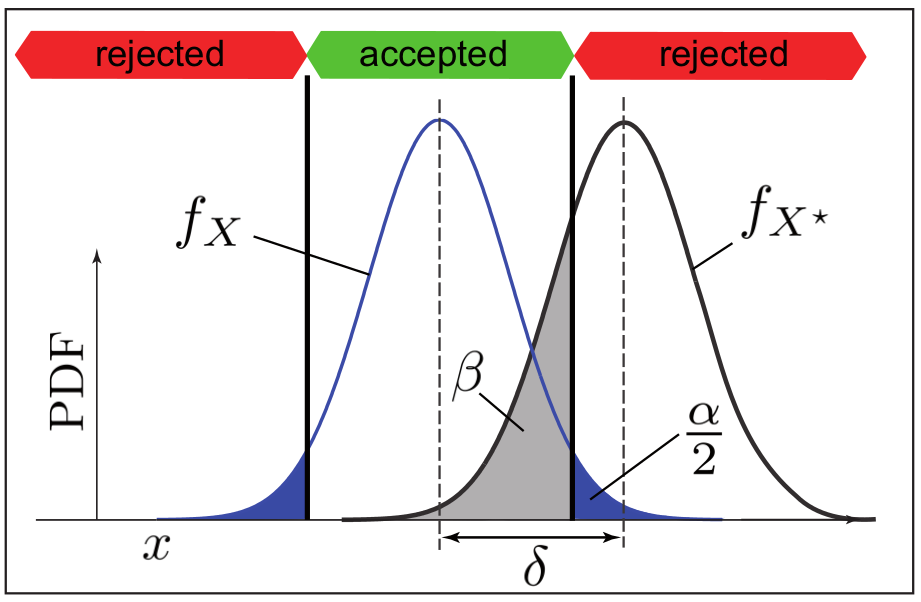
\includegraphics[trim = 0mm 0mm 0mm 2mm, clip, width=0.6\textwidth]{figures/SebastianNotesScreenshots/Screenshot2020-02-21t14-58-49.png} 
	\caption{Relationship between $\alpha$, $\beta$, and $\delta$}
	\label{Fig:AlphaaBetaDelta}
\end{figure}

Common values are $\alpha = 0.01$ and $\beta = 0.05$. Figure B.3 provides a visual representation of the ``no blunder'' (i.e. null) and ``blunder'' hypotheses. Both hypotheses are assumed to have Gaussian (i.e. standard, or normal) distribution, and the blunder hypothesis has a non-zero mean value. That non-zero mean value, also equal to the distance between the center of each distribution, is referred to as the ``non-centrality parameter'' $\delta_0$. For $\alpha = 0.01$ and $\beta = 0.05$, the non-centrality parameter is $\delta_0 = 4.22068$. 

To compute the minimum detectable bias, the minimum gross error $\nabla Y_i$ is set equal to the gross error $\Delta \hat{Y}_i$ which produces a test statistic $T_N$ equal to $\delta_0$:
\begin{equation}\label{eq:MinDetectBlunder1}
T_N = \Delta \hat{Y}_i / \sigma_{\Delta \hat{Y}_i} = \delta_0
\end{equation}

However, instead of setting $\sigma_{\Delta \hat{Y}_i}$ equal to the expression for $\sigma_{\Delta Y_i}$ provided by equation \ref{eq:SigmaY} to derive the final expression for $T_N$, a slightly different expression is used:
\begin{equation}\label{eq:SigmaYv2}
\sigma_{\Delta \hat{Y}_i} = \frac{\text{MCov}_{ii}}{\sqrt{Q_{RR,ii}}}
\end{equation}
where the $\sqrt{\text{APV}}$ term has been removed. Why is $\sqrt{\text{APV}}$ not employed? Leick \cite{leick} provides an explanation: ``Baarda’s (1967) development of the concept of reliability of networks is based on un-Studentized hypothesis tests, which means that the a priori variance of unit weight is assumed to be known. Consequently, the a priori variance of unit weight (not the a posteriori variance of unit weight) is used in this section.'' The a priori variance of unit weight is assumed equal to identity, and thus the expression is simplified to the form in equation \ref{eq:SigmaYv2}. A significant benefit of this revision is that the internal reliability metric (and thus the external reliability metric as defined in section \ref{sec:ExtRel}) for each observation is not dependent on any actual observations collected in the field, and thus can serve as a powerful planning tool prior to the survey.

The minimum detectable bias is then computed as:
\begin{equation}\label{eq:MinDetectBlunder2}
\begin{split}
\nabla \hat{Y_i} &= \delta_0 \; \sigma_{\Delta \hat{Y}_i} \\
&= \delta_0 \; \frac{\text{MCov}_{ii}}{\sqrt{Q_{RR_{ii}}}} \\
&= \delta_0 \; \frac{\text{MCov}_{ii}}{\sqrt{Q_{RR_{ii}}}} \frac{Q_{RR_{ii}}}{\text{MCov}_{ii}} \frac{1}{r_i} \\
&= \delta_0 \; \frac{\sqrt{Q_{RR_{ii}}}}{r_i}\\
&= \delta_0 \; \frac{\sqrt{r_i \; \text{MCov}_{ii}}}{r_i}\\
&= \delta_0 \; \frac{\sqrt{\text{MCov}_{ii}}}{\sqrt{r_i}}
\end{split}
\end{equation}

For a given $\delta_0$ and $\text{MCov}_{ii}$, a larger redundancy number means a smaller minimum detectable bias. In other words, the minimum detectable bias is inversely proportional to the square root of the individual redundancy value. An observation with low redundancy and thus a large minimum detectable bias can potentially significantly derail the estimated state (i.e. adjusted position), as illustrated in section \ref{sec:RelExamples}.

\section{External Reliability} \label{sec:ExtRel}

External reliability is calculated by mapping the minimum detectable blunders for each observation through the state update operation, which provides the impact on the estimated state from that blunder:

\begin{equation}\label{eq:MapMinDetBlunderToState}
\nabla \hat{\textbf{x}}_i = \left( H^T \; \text{MCov}^{-1} \; H \right)^{-1} H^T \; \text{MCov}^{-1} \; \nabla \hat{\textbf{Y}}_i
\end{equation}

where $\nabla \hat{\textbf{Y}}_i$ is a vector of m elements which are all equal to zero except the $i^{\text{th}}$ element, which has value $\nabla \hat{Y}_i$:

\begin{equation}\label{eq:eq:MapMinDetBlunderToState3}
\nabla \hat{\textbf{Y}}_i = \begin{bmatrix}
0 & \ldots & 0 & \nabla \hat{Y}_i & 0 & \ldots & 0
\end{bmatrix}^T
\end{equation}

The result is an array of ``state impact'' vectors, one for each observation. Lower redundancy leads to a larger minimum detectable bias, which in turn leads to larger state impact vectors. 

To visualize these state impact vectors, a ''Reliability Rectangle'' is constructed, as illustrated in figure \ref{Fig:RR}. This rectangle allows the user to quickly grasp the effect that strong or weak redundancy in the observations has on the final state. The result is intuitive and actionable information for the surveyor regarding the susceptibility of any planned or collected observations to blunders or significant outliers.

A reliability rectangle is defined by the following properties:
\begin{itemize}
    \item The rectangle is centered at the estimated state position (or the a priori position if the survey has not yet been conducted)
    \item All external reliability vectors are rotated into the ENU frame, using the above center position as the reference position for that rotation
    \item The rectangle is oriented such that the major axis direction matches the direction of the largest magnitude state vector, and the scaling of the rectangle in that direction matches the magnitude of the largest magnitude state vector
    \item The smaller dimension of the rectangle is scaled to fit all the other external reliability vectors
\end{itemize}

\begin{figure}[!htb]
	\centering
	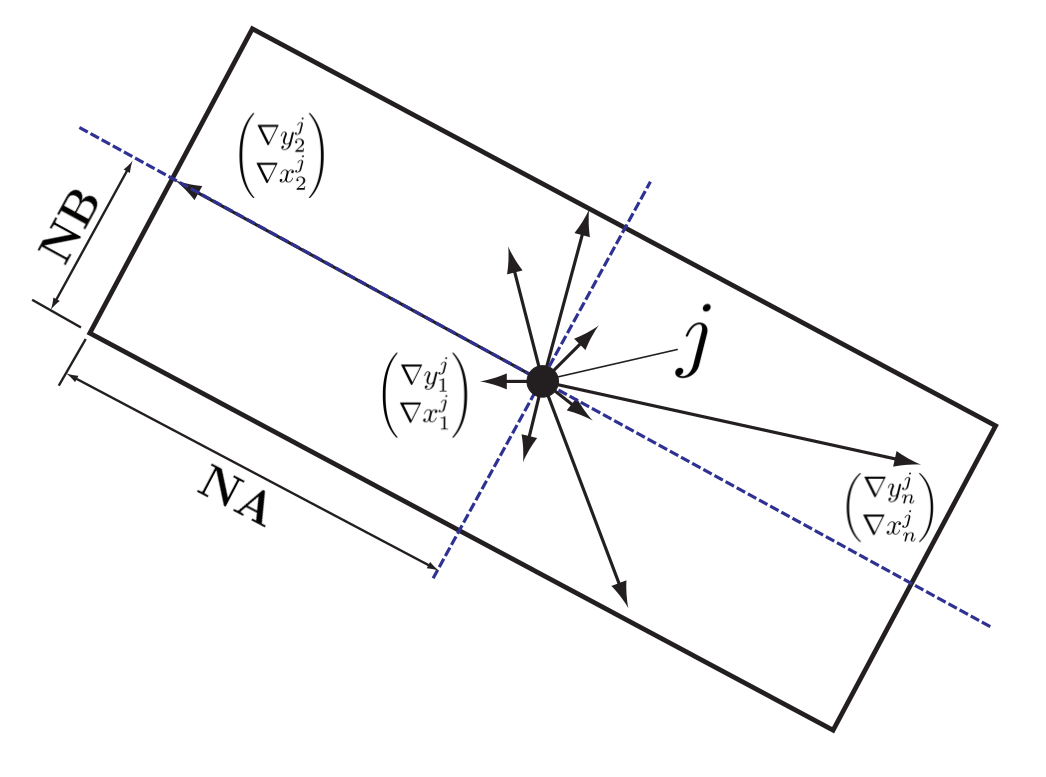
\includegraphics[trim = 0mm 0mm 0mm 2mm, clip, width=0.8\textwidth]{figures/SebastianNotesScreenshots/Screenshot2020-02-24t09-52-28.png} 
	\caption{Example reliability rectangle}
    \label{Fig:RR}
\end{figure}

\newpage

\section{Examples} \label{sec:RelExamples}

Below are two ``toy problems'' that illustrate the utility of the above metrics for surveyors. While a typical survey has many more observations than these simple examples, employing relatively few  observations in these examples hopefully allows the reader to more easily grasp the nature of the reliability metrics and how they are computed for each observation.

\subsection{Range Example}

The first simple example employs range observations from several stations to estimate a desired position, as illustrated by figure \ref{Fig:Ex1Map}. Note that the example contains no specific distance units. The position of interest is located at [0,10], with the true position matching the a priori nominal position to simplify the example. The ranging station positions are fixed at [0,0], [1,0], and [10,10]. Measurement noise of 0.01 1-$\sigma$ is added to the observations, and a measurement uncertainty of 0.01 1-$\sigma$ is employed in the estimation process (and thus all measurements have equal weight).

\newpage

\begin{figure}[!htb] 
	\centering
	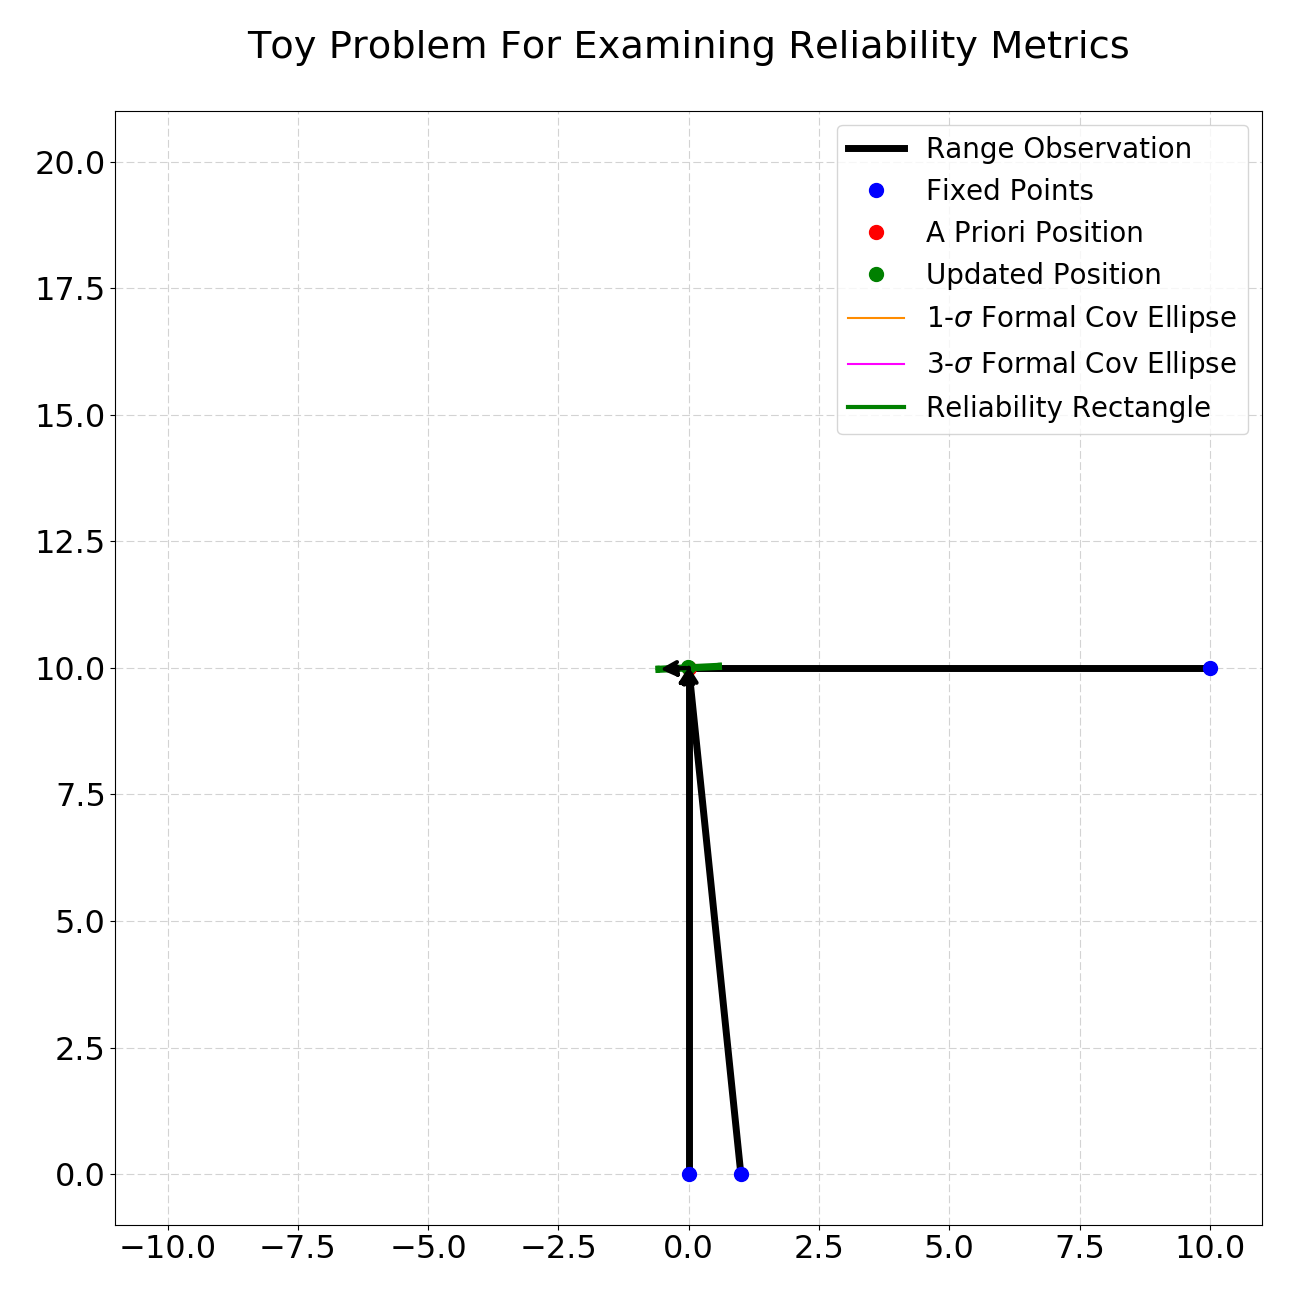
\includegraphics[trim = 0mm 0mm 0mm 5mm, clip, width=0.9\textwidth]{figures/ReliabilityExample/v10/Map.png}
	\caption{Ranging example - map}
    \label{Fig:Ex1Map}
\end{figure}

\newpage

Figure \ref{Fig:Ex1MapZoom} provides a zoomed-in view of the region around the point of interest. The formal uncertainty is visible via the 3-$\sigma$ formal covariance ellipse, which appears reasonably sized in both directions. In contract, the magnitude of the reliability rectangle is large in the East-West direction - far larger than the formal covariance scaling in the East-West direction. The lack of redundancy in the East-West direction from having only one ranging station to the East of the estimated position results in a large reliability rectangle magnitude.

\begin{figure}[!htb]
	\centering
	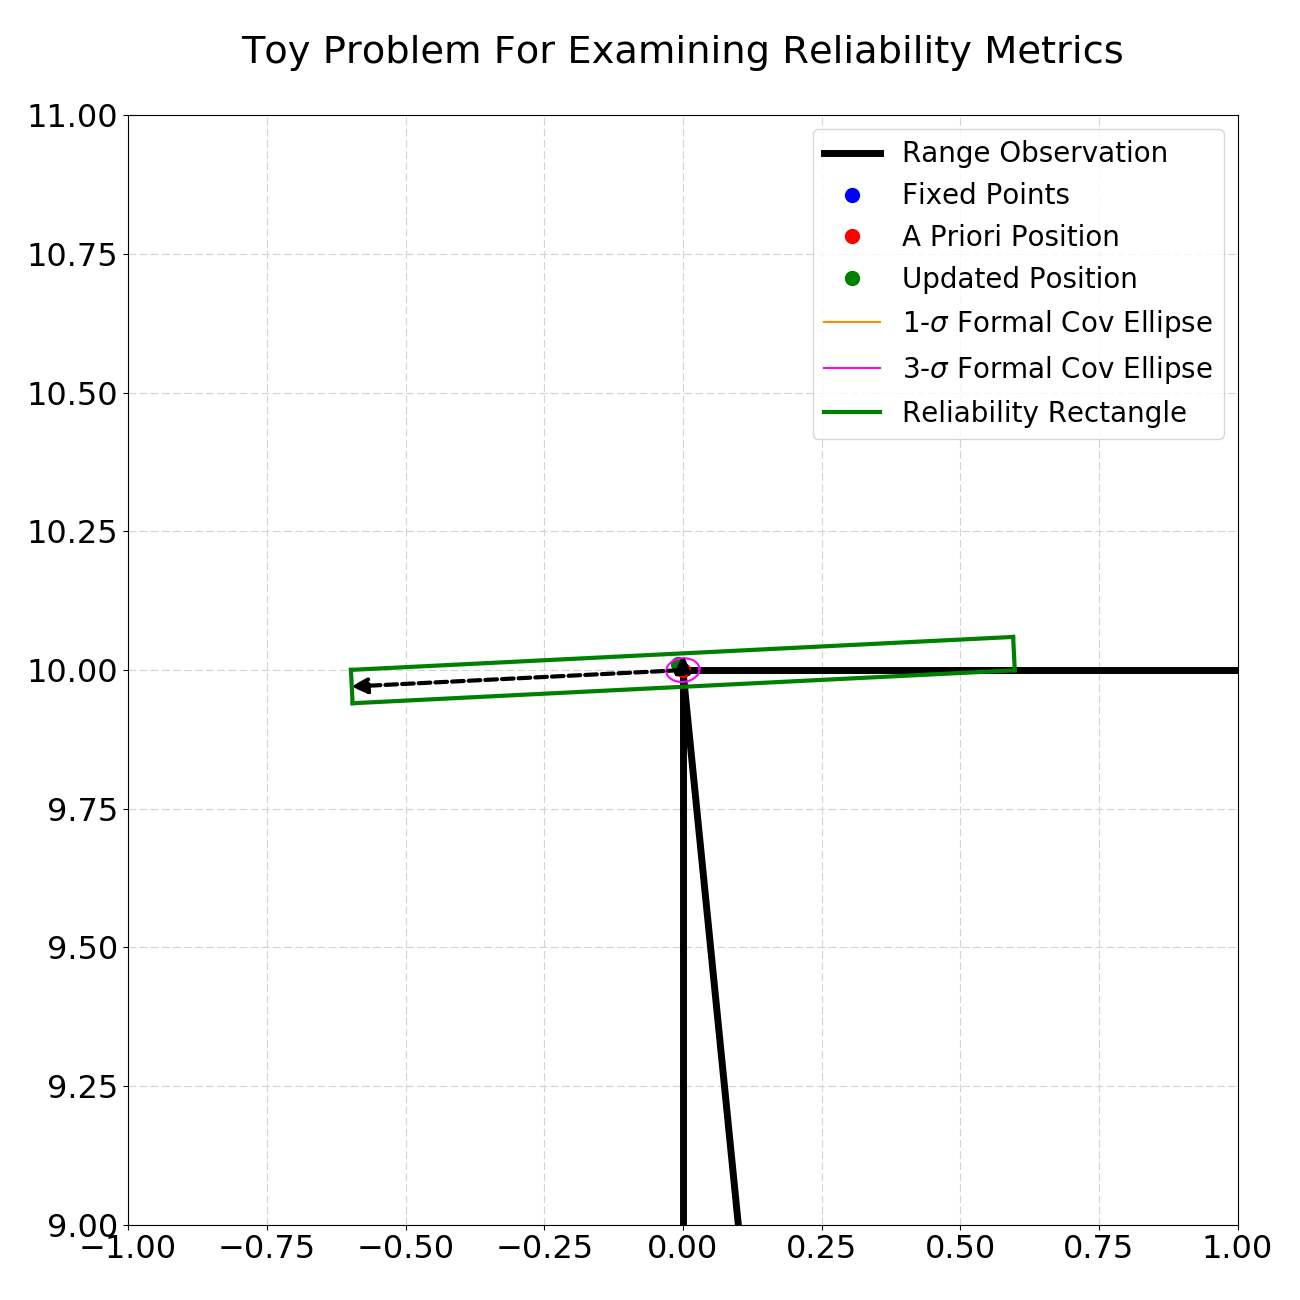
\includegraphics[trim = 0mm 0mm 0mm 5mm, clip, width=0.9\textwidth]{figures/ReliabilityExample/v10/MapZoomed.png}
	\caption{Ranging example - zoomed map}
    \label{Fig:Ex1MapZoom}
\end{figure}

\newpage

To demonstrate what a reliability rectangle illustrates, the minimum detectable bias computed for the East station range observation is added to that observation, as shown in figure \ref{Fig:Ex1MapZoomBlunder}. The result: the estimated position now lies approximately on the western edge of the reliability rectangle. (The estimated position lands exactly on the edge if no measurement noise is added.)

\begin{figure}[!htb]
	\centering
	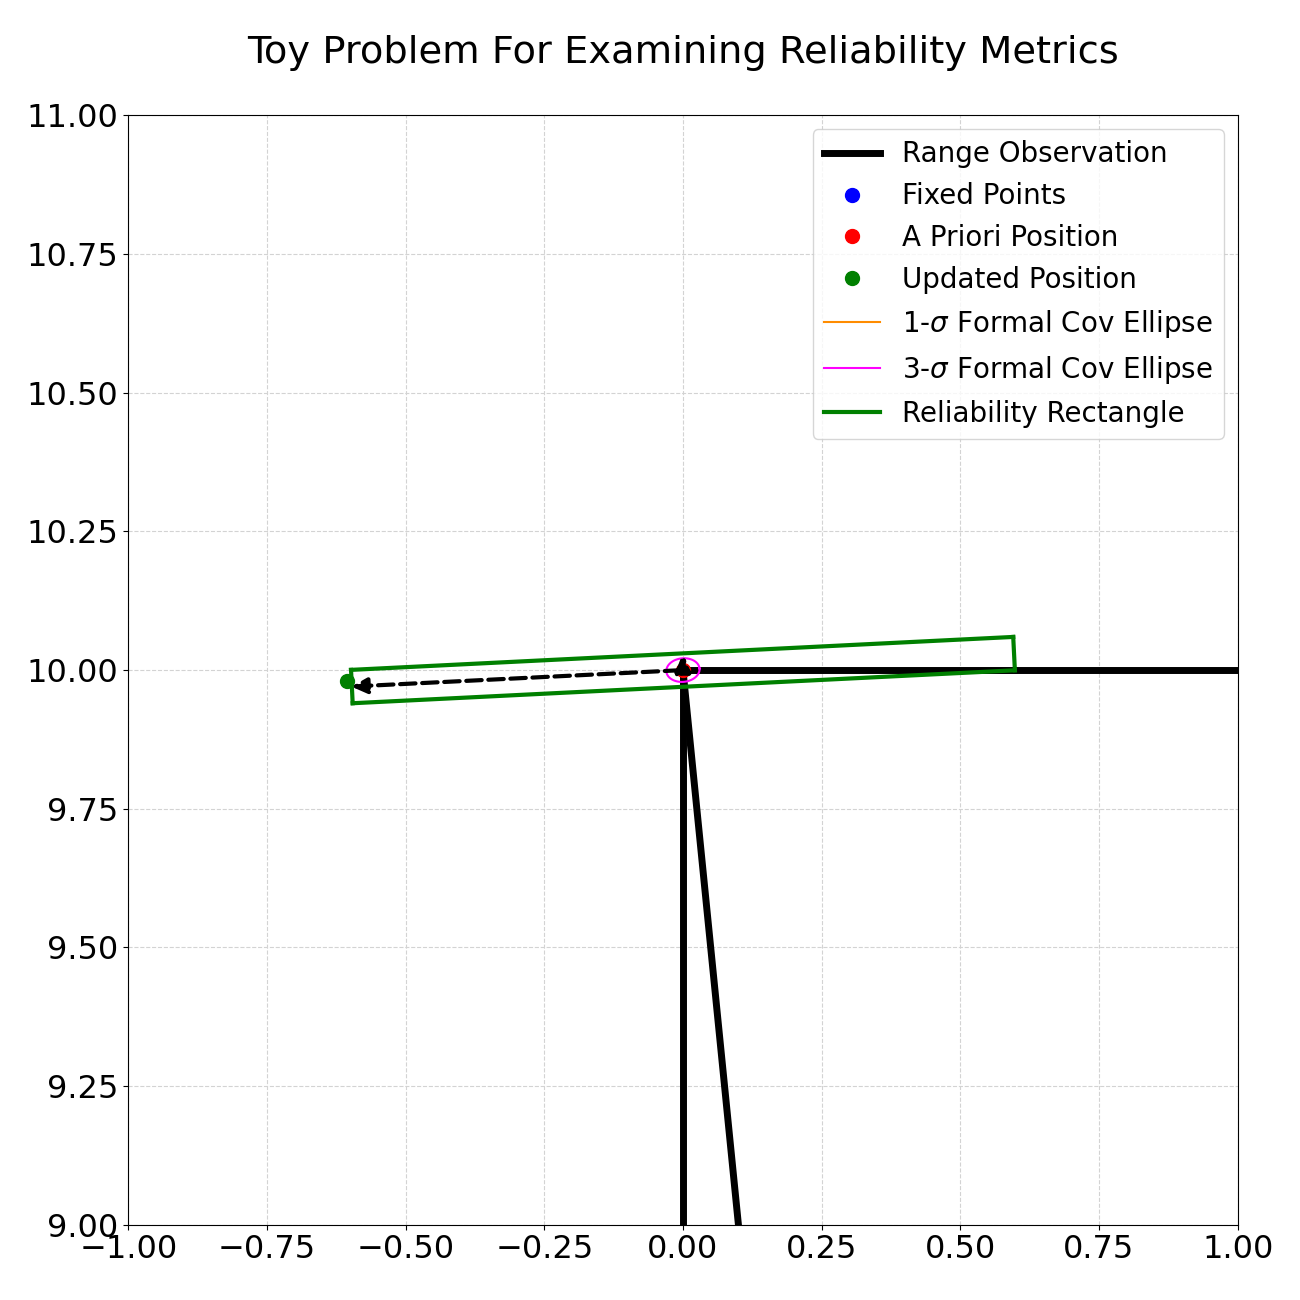
\includegraphics[trim = 0mm 0mm 0mm 5mm, clip, width=0.9\textwidth]{figures/ReliabilityExample/v13/MapZoomed.png}
	\caption{Ranging example - east station blunder}
    \label{Fig:Ex1MapZoomBlunder}
\end{figure}

\newpage

To illustrate how the estimated position is so heavily affected by a blunder in a low redundancy observation, each of the ranging observations can be viewed as a circle with radius equal to the range value, as shown in figure \ref{Fig:Ex1MapObs}:

\begin{figure}[!htb]
    \centering
    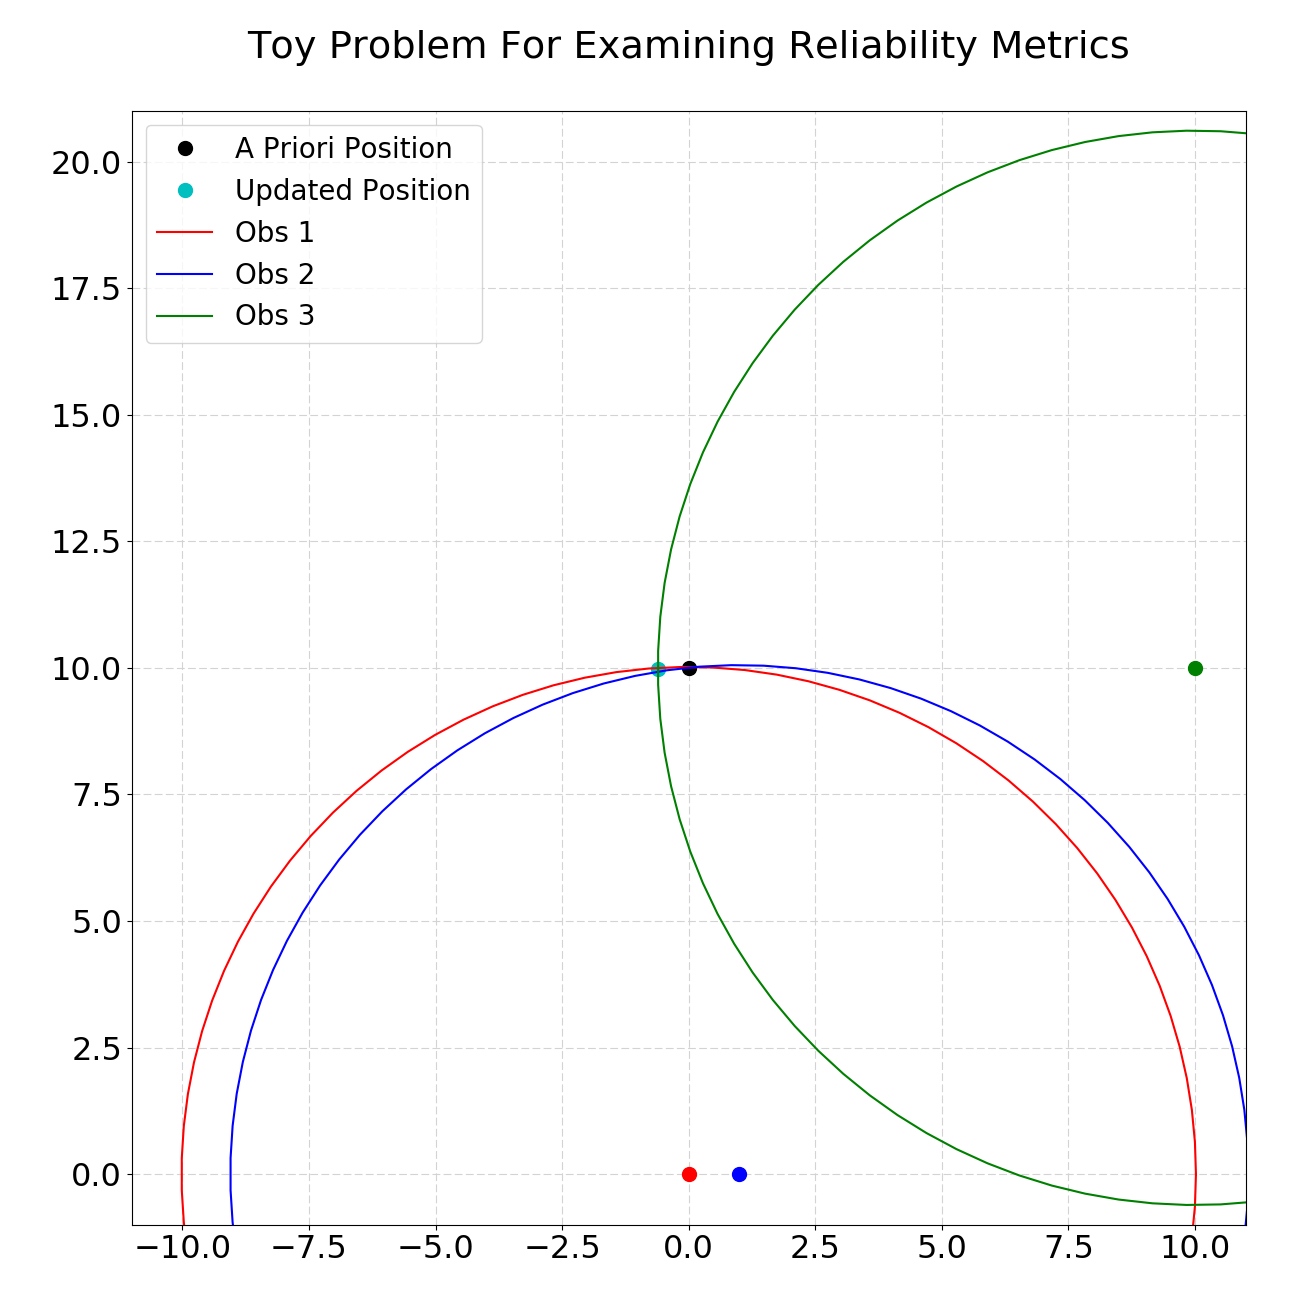
\includegraphics[trim = 0mm 0mm 0mm 0mm, clip, width=1.0\textwidth]{figures/ReliabilityExample/v53/MapObs.png}
    \caption{Ranging example - observations as circles}
    \label{Fig:Ex1MapObs}
\end{figure}


\newpage

Zooming in on the point of interest, figure \ref{Fig:Ex1MapObsZoomed} shows the estimated position is now 0.6 units to the west, just as in figure \ref{Fig:Ex1MapZoomBlunder}. The least squares estimation process identifies the position that minimizes the sum of the squared pre-fit residuals, which means the estimated position lies on the ``Obs 3'' line between the ``Obs 1'' and ``Obs 2'' lines - the best place to minimize those residuals. The low redundancy of the east station observation allows this large blunder to significantly affect the state.

\begin{figure}[!htb]
    \centering
    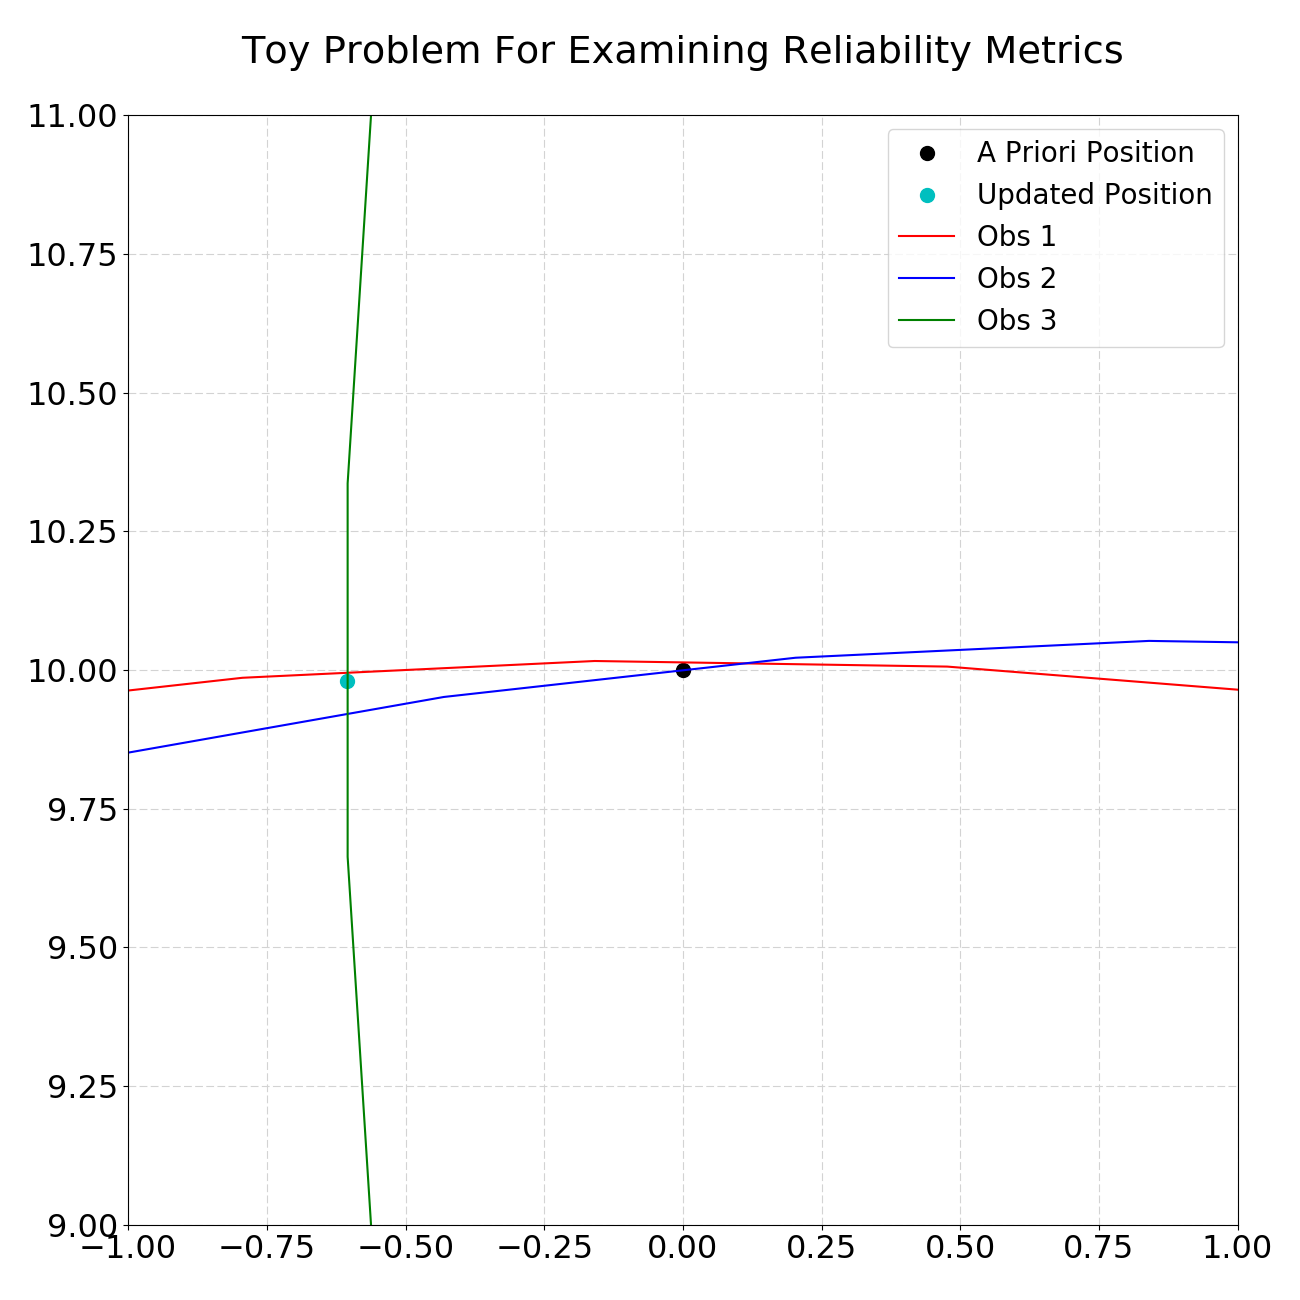
\includegraphics[trim = 0mm 0mm 0mm 0mm, clip, width=1.0\textwidth]{figures/ReliabilityExample/v53/MapObsZoomed.png}
    \caption{Ranging example - observations as circles}
    \label{Fig:Ex1MapObsZoomed}
\end{figure}

%MapObsZoomed.png


 
\newpage

The pre-fit and post-fit observation residuals for the blunder scenario are provided in figures \ref{Fig:Ex1PrefitRes} and \ref{Fig:Ex1PostfitRes}. Note that while the third pre-fit residual (corresponding to the East station range observation) is clearly the largest residual, the third post-fit residual is reasonably close to zero and smaller than the other two residuals. Thus an analysis of the post-fit residuals can easily miss any blunders or outliers in observations that have poor redundancy, and these blunders or outliers can also lead to the rejection of good observations if the surveyor does not address this lack of redundancy (e.g. throwing out observation two in this scenario, as it has the largest magnitude post-fit residual).

%\newpage
\begin{figure}[!htb]
	\centering
	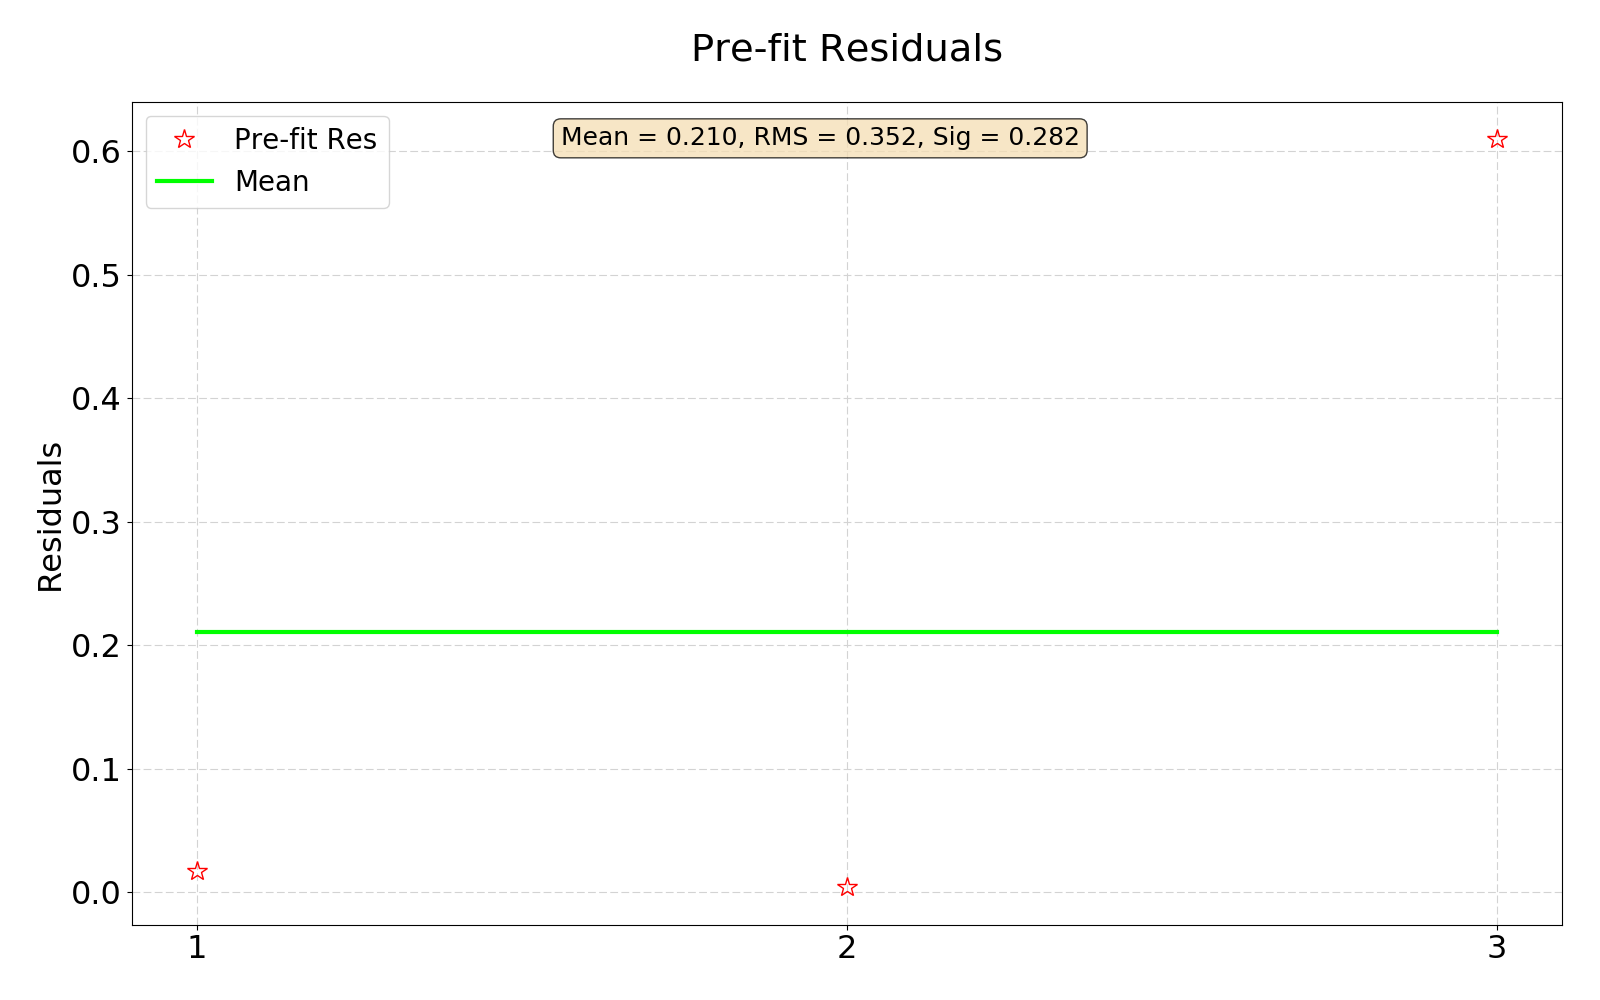
\includegraphics[trim = 0mm 0mm 0mm 0mm, clip, width=1.0\textwidth]{figures/ReliabilityExample/v53/PrefitResiduals.png}
	\caption{Ranging example - east station blunder pre-fit residuals}
    \label{Fig:Ex1PrefitRes}
\end{figure}

\newpage
\begin{figure}[!htb]
	\centering
	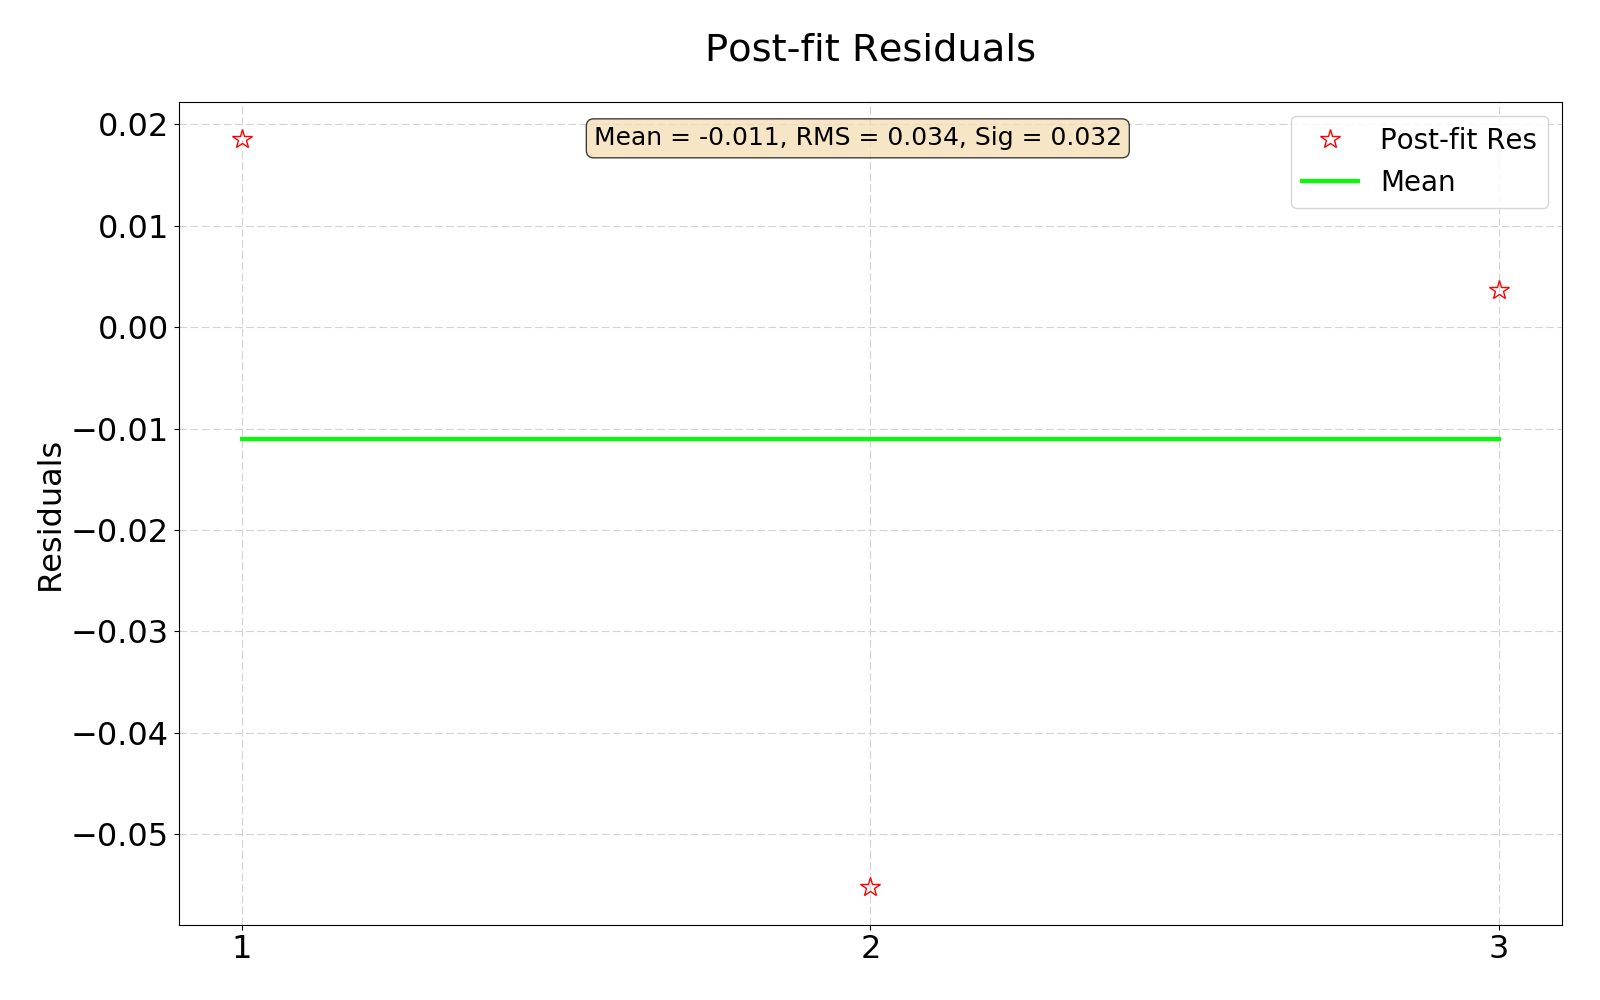
\includegraphics[trim = 0mm 0mm 0mm 0mm, clip, width=1.0\textwidth]{figures/ReliabilityExample/v53/PostfitResiduals.png}
	\caption{Ranging example - east station blunder post-fit residuals}
    \label{Fig:Ex1PostfitRes}
\end{figure}

\newpage

The redundancy values (local reliability) for the three observations highlight how the third observation has almost no redundancy, as shown in figure \ref{Fig:Ex1redundancy}.

\begin{figure}[!htb]
	\centering
	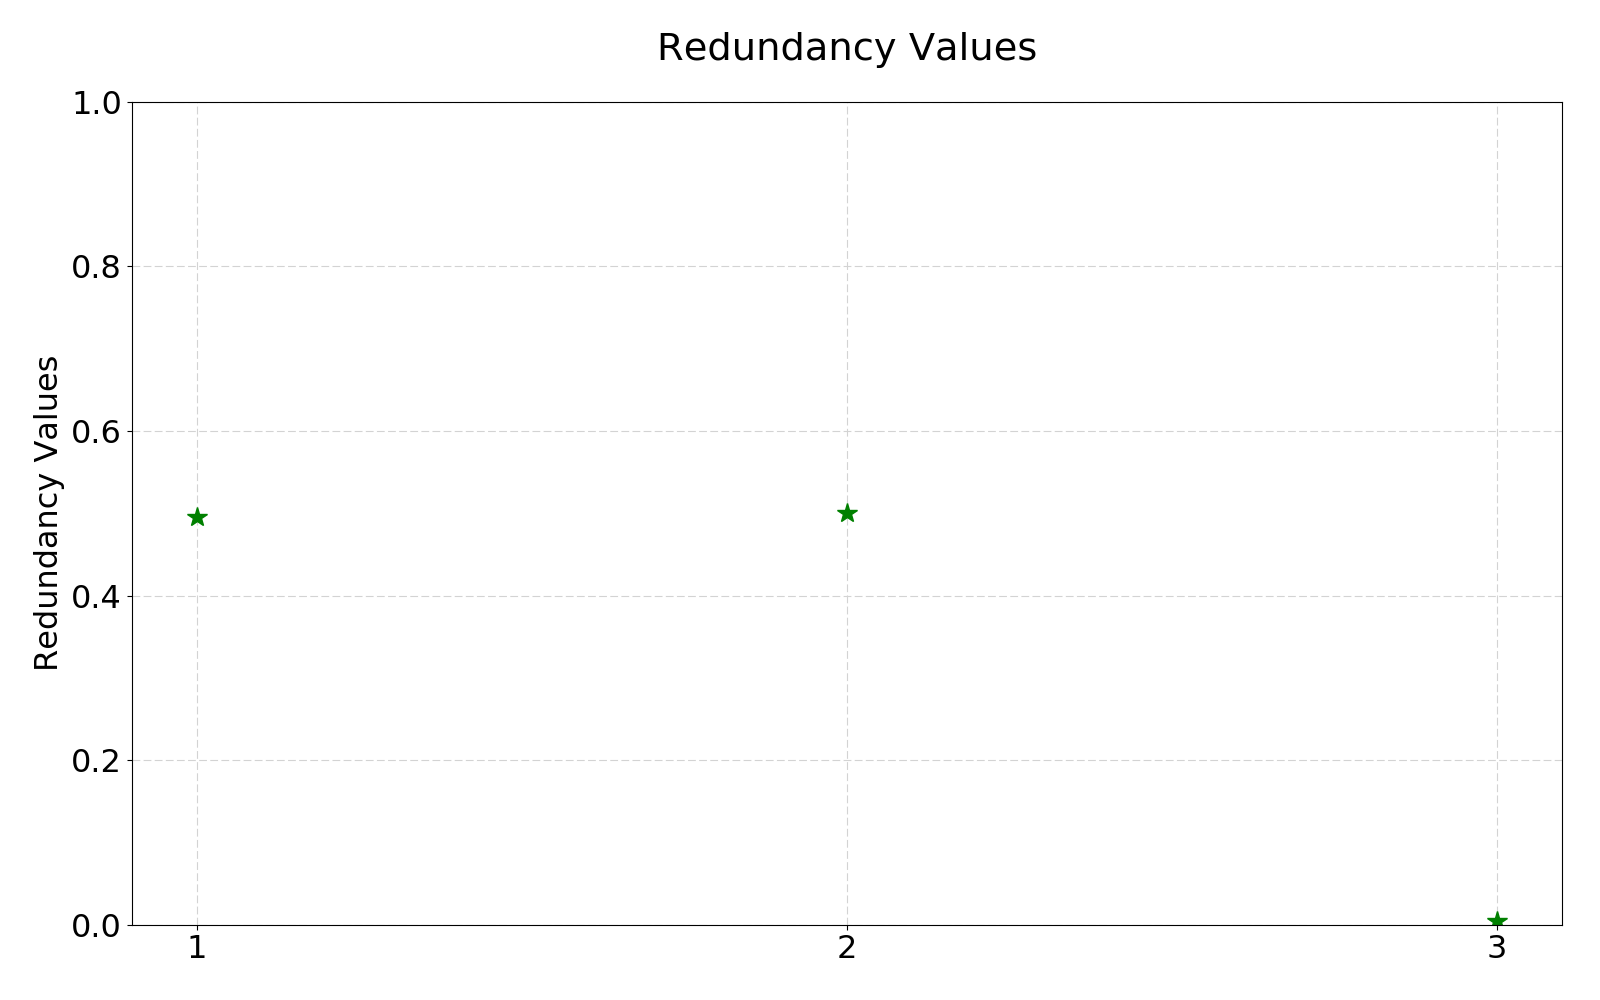
\includegraphics[trim = 0mm 0mm 0mm 0mm, clip, width=1.0\textwidth]{figures/ReliabilityExample/v53/Redundancy.png}
	\caption{Ranging example - redundancy values}
    \label{Fig:Ex1redundancy}
\end{figure}

\newpage

The minimum detectable bias values (internal reliability) for the three observations, as shown in figure \ref{Fig:Ex1minDetBias}, reveals how the third observation has a significantly larger magnitude due to the poor redundancy of that observation:

\begin{figure}[!htb]
	\centering
	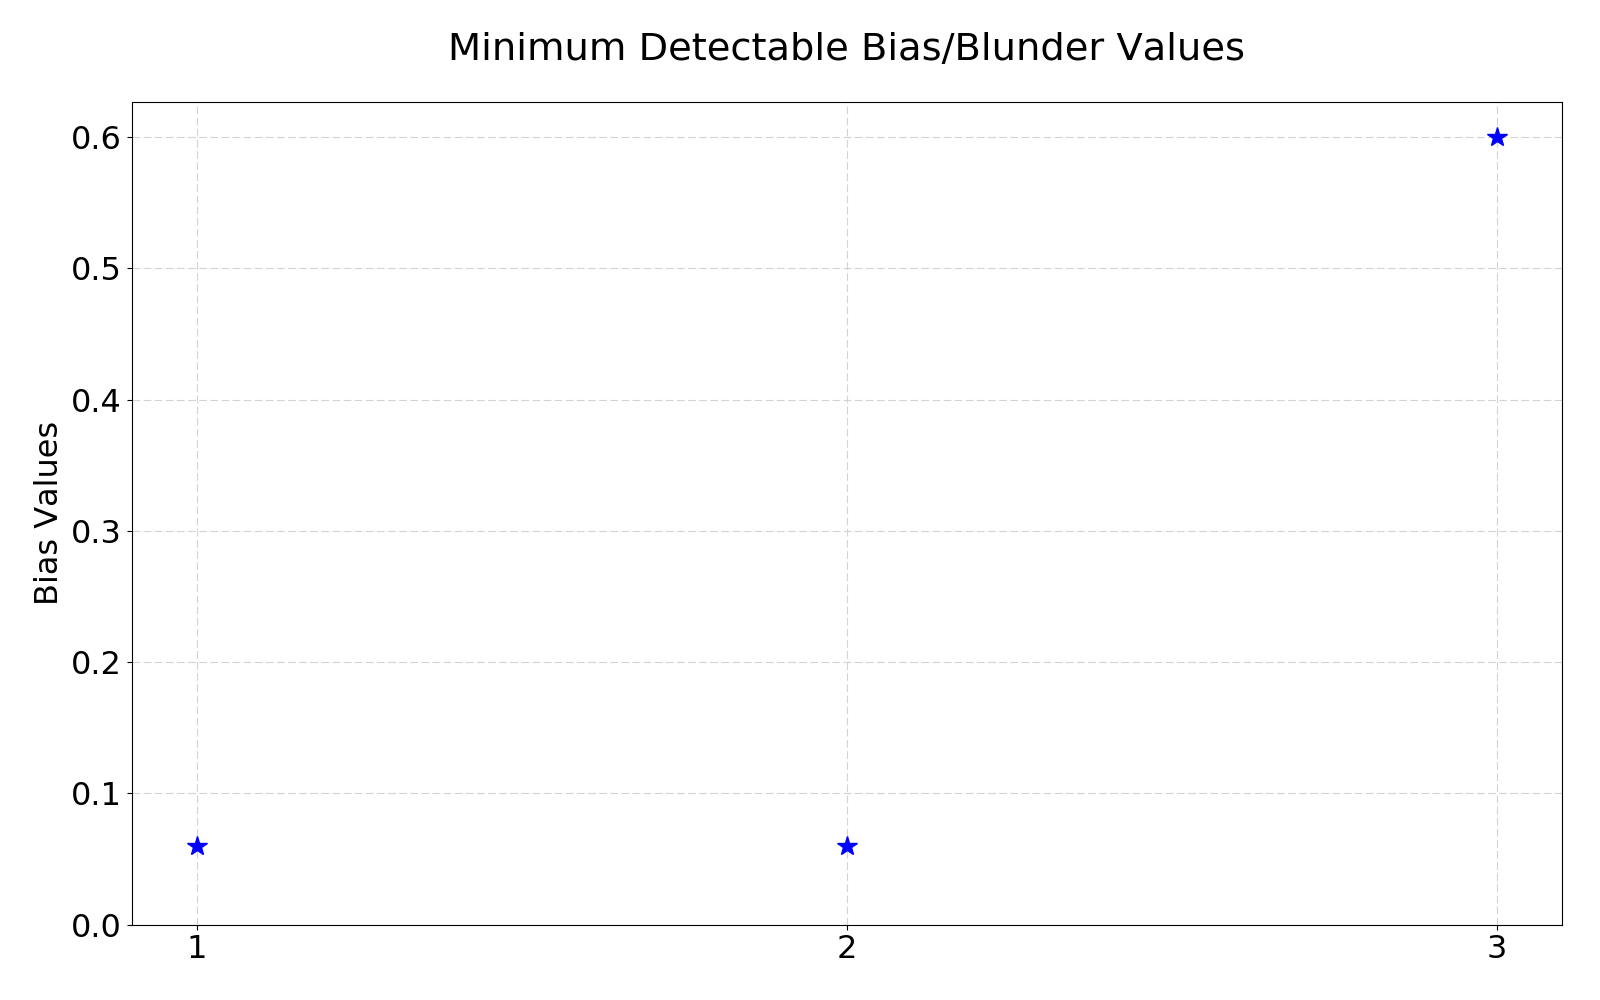
\includegraphics[trim = 0mm 0mm 0mm 0mm, clip, width=1.0\textwidth]{figures/ReliabilityExample/v53/MinDetBias.png}
	\caption{Ranging example - minimum detectable bias values}
    \label{Fig:Ex1minDetBias}
\end{figure}

\newpage

The external reliability vector magnitudes for the three observations, as shown in figure \ref{Fig:Ex1ExtVectMag}, similarly shows the third observation has a much larger magnitude than the other two observations:

\begin{figure}[!htb]
	\centering
	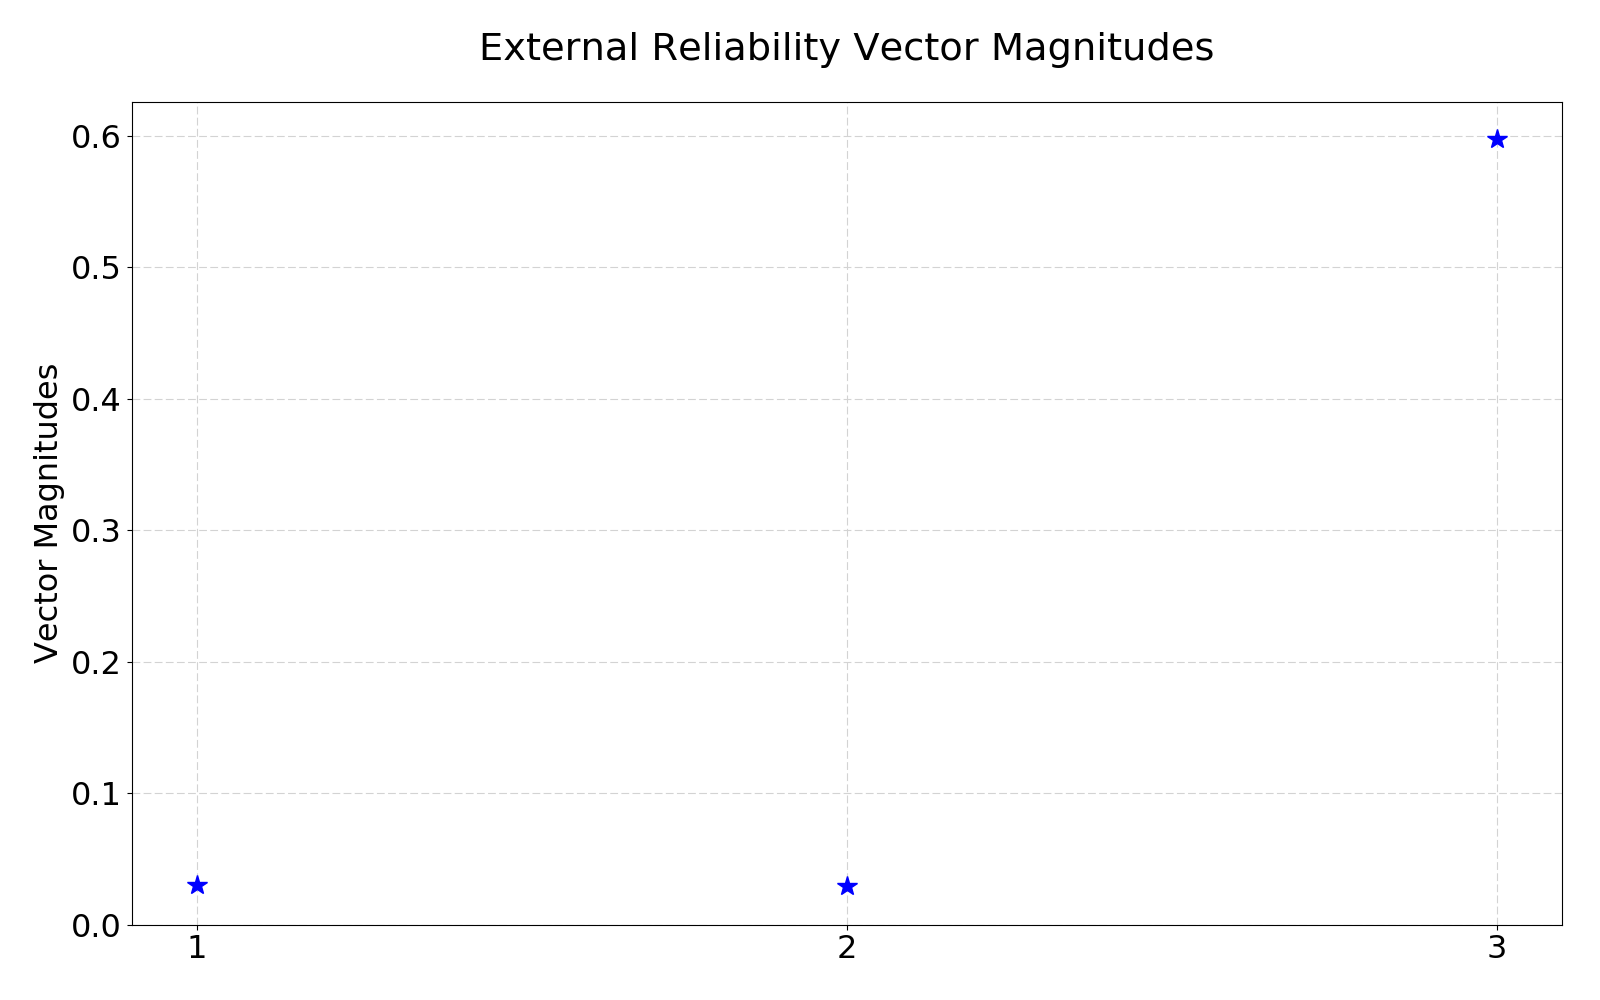
\includegraphics[trim = 0mm 0mm 0mm 0mm, clip, width=1.0\textwidth]{figures/ReliabilityExample/v53/ExtRelVectMags.png}
	\caption{Ranging example - external reliability vector magnitudes}
    \label{Fig:Ex1ExtVectMag}
\end{figure}

\newpage

The post-fit residuals plotted in figure \ref{Fig:Ex1PostfitRes} can be transformed into standard residuals, as described in section \ref{sect:StdRes}. The results are provided in figure \ref{Fig:Ex1StdRes}. Note that even though the observation 3 has the blunder, the largest standard residual magnitude occurs for observation 2. Thus if the surveyor only checks the standard residual magnitudes and ignores the redundancy, internal reliability, and external reliability metrics, a good observation can be excluded and a blunder can remain. In other words, standard residuals can prove unreliable in identifying blunders if sufficient redundancy is not established for all observations.

\begin{figure}[!htb]
	\centering
	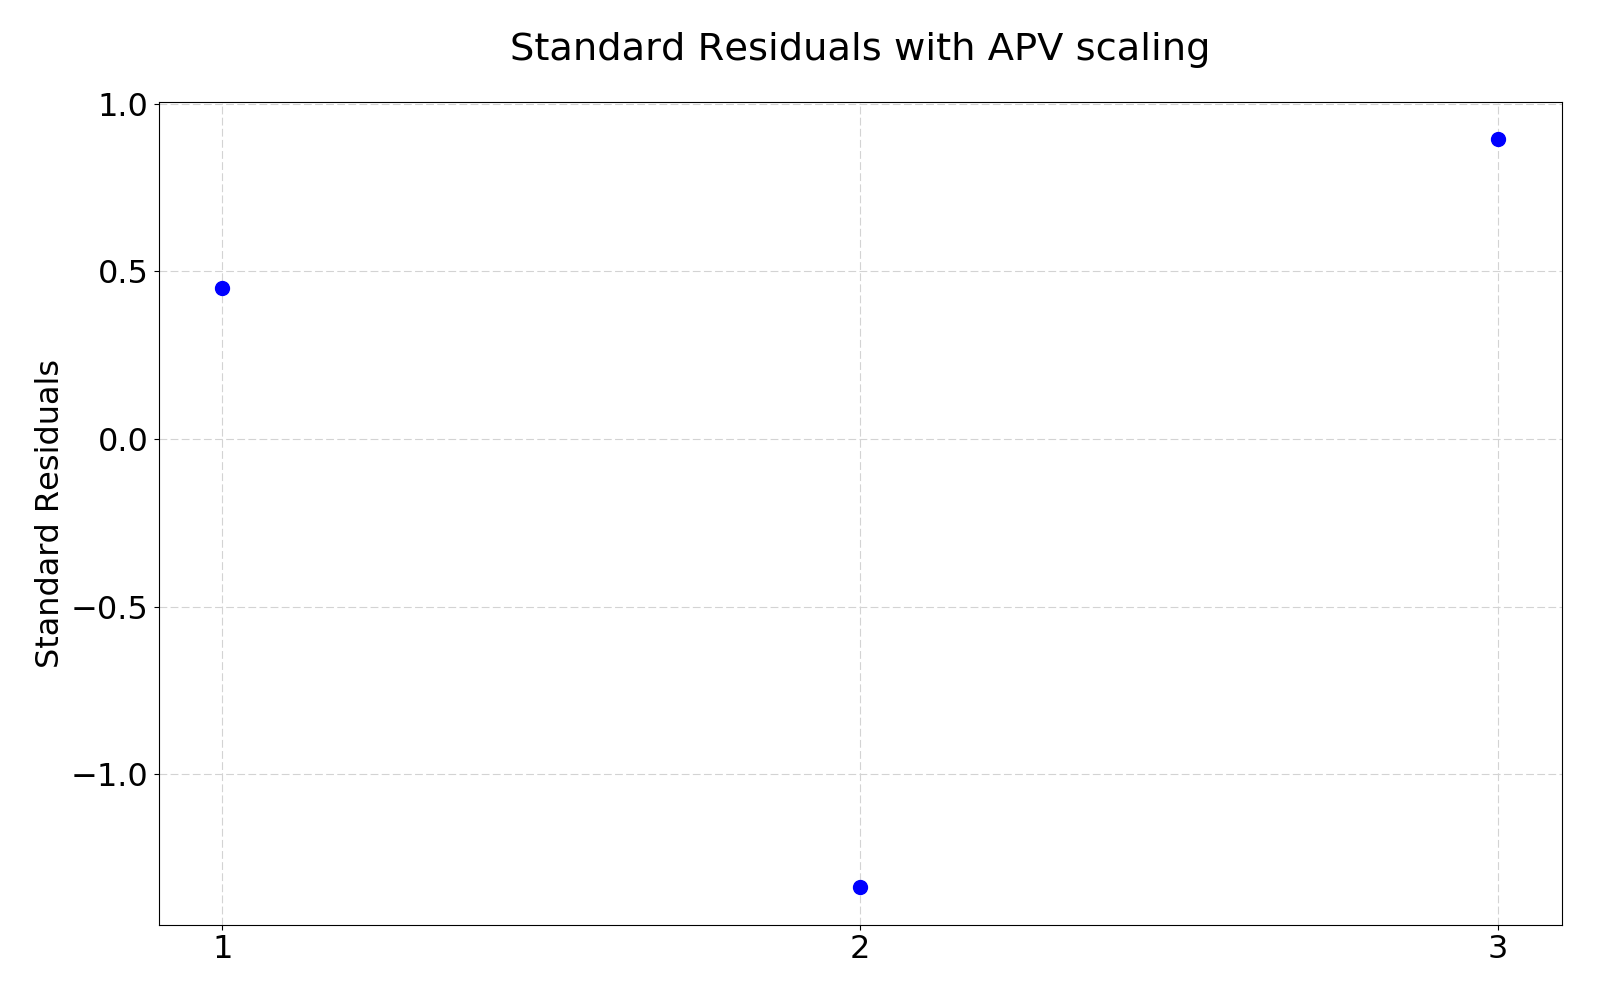
\includegraphics[trim = 0mm 0mm 0mm 0mm, clip, width=1.0\textwidth]{figures/ReliabilityExample/v54/StandardResidualsWithAPV.png}
	\caption{Ranging example - standard residuals with east station blunder}
    \label{Fig:Ex1StdRes}
\end{figure}

\newpage
Given the wide reliability rectangle presented in figure \ref{Fig:Ex1MapZoom}, a good course of action is to add observations that provide redundancy in the east-west direction. Figure \ref{Fig:Ex1AddedObsMap} illustrates the result of adding two ranging stations to the east (neither of which contain blunders, but the blunder for observation 3 remains):

\begin{figure}[!htb]
	\centering
	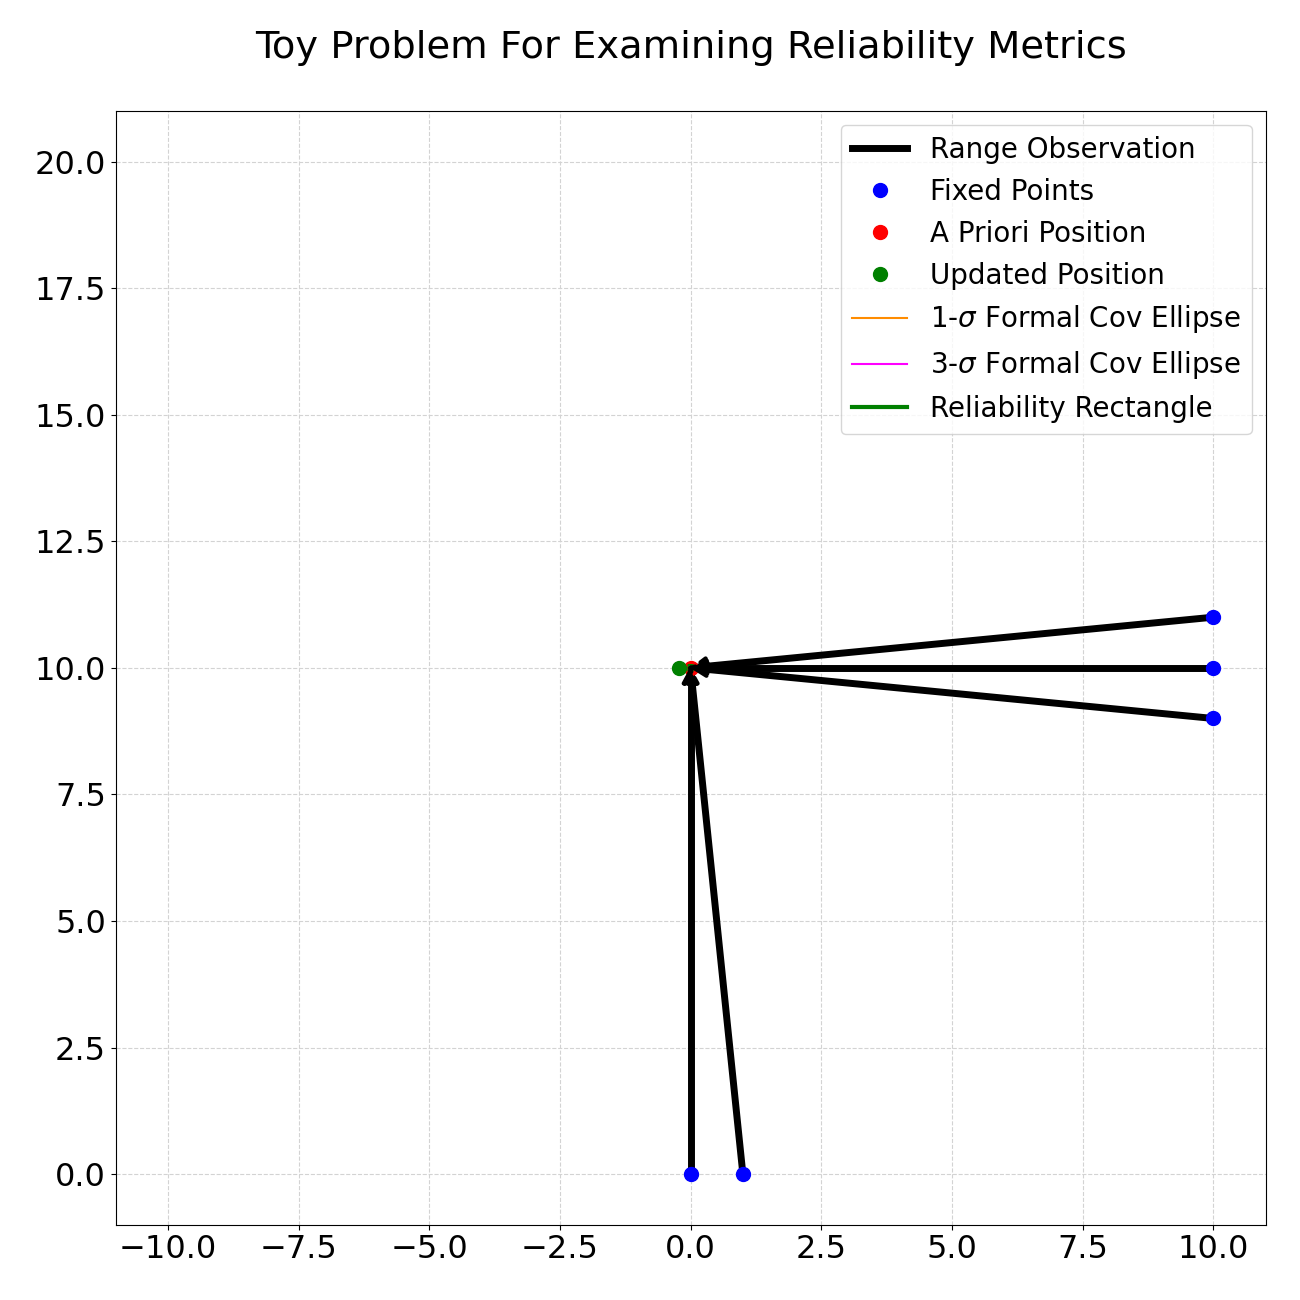
\includegraphics[trim = 0mm 0mm 0mm 5mm, clip, width=0.9\textwidth]{figures/ReliabilityExample/v15/Map.png}
	\caption{Ranging example - adding additional observations}
    \label{Fig:Ex1AddedObsMap}
\end{figure}

\newpage
Zooming in on the point of interest, figure \ref{Fig:Ex1AddedObsMapZoomed} shows the estimated position is approximately 0.2 units to the west, rather than 0.6 as seen in figure \ref{Fig:Ex1MapObsZoomed}. The positive influence of the additional measurements results in a smaller impact on the estimated state from the observation 3 blunder.

\begin{figure}[!htb]
	\centering
	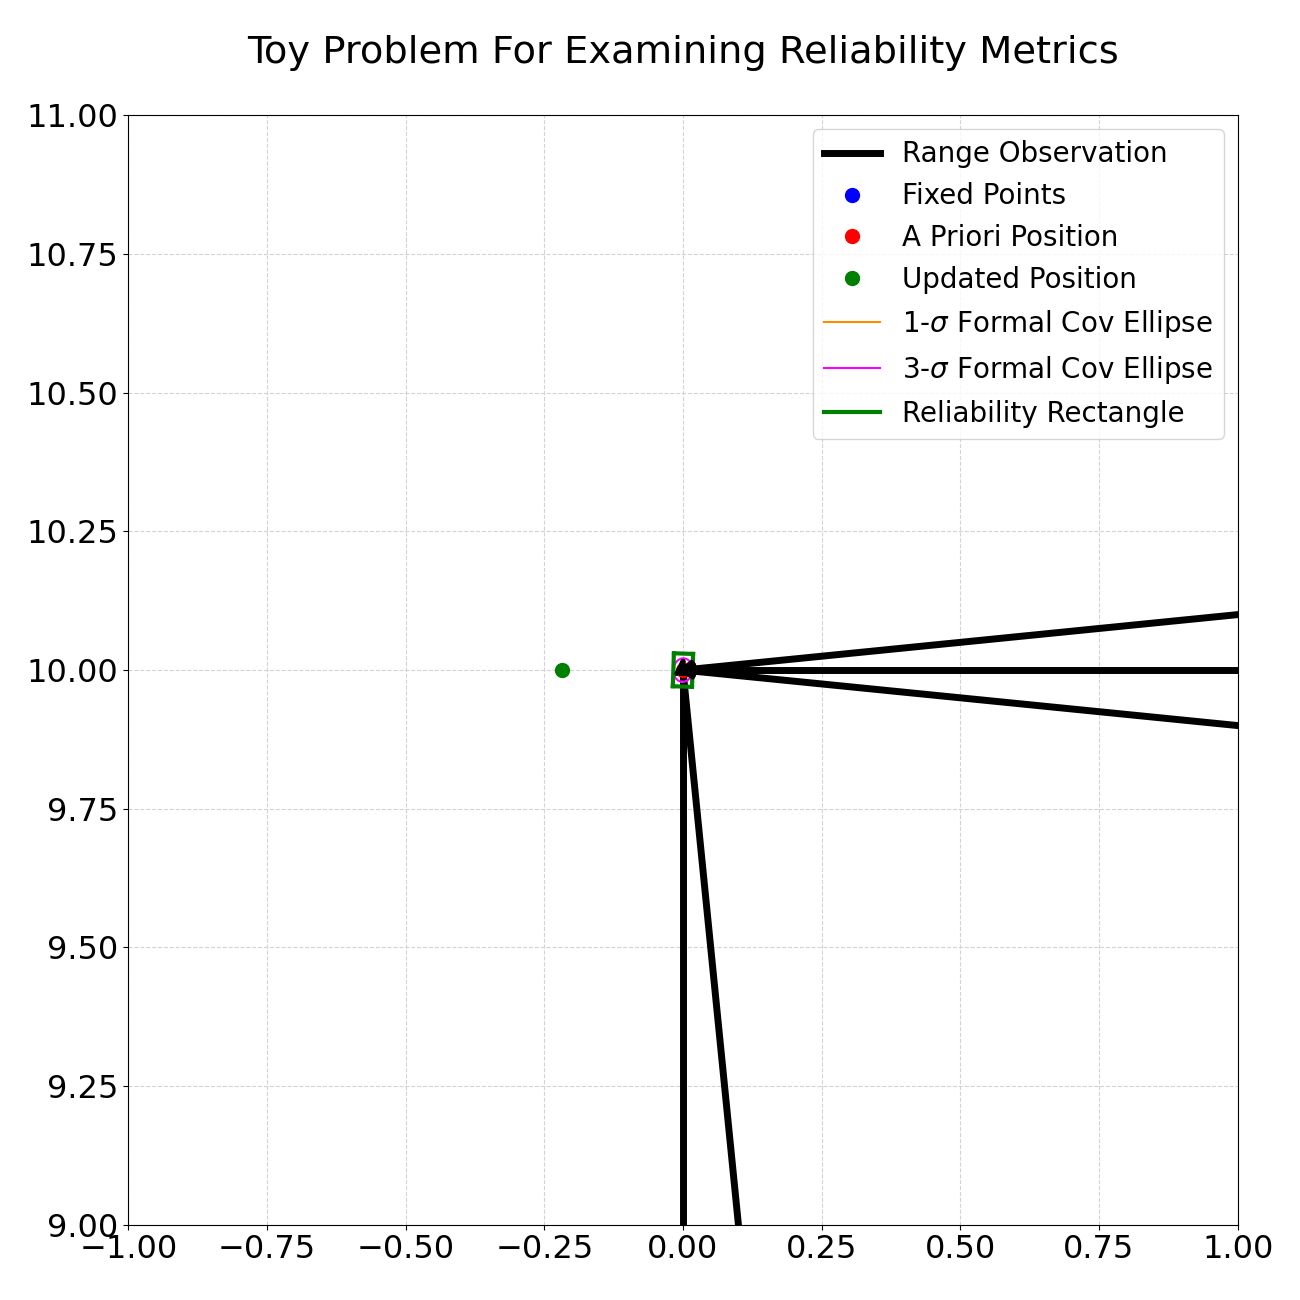
\includegraphics[trim = 0mm 0mm 0mm 5mm, clip, width=0.9\textwidth]{figures/ReliabilityExample/v15/MapZoomed.png}
	\caption{Ranging example - adding additional observations - zoomed}
    \label{Fig:Ex1AddedObsMapZoomed}
\end{figure}

\newpage

Now that all observations have reasonable redundancy, the standard residuals now correctly identify the blunderous observation, as shown in figure \ref{Fig:Ex1AddedObsStdRes}.

\begin{figure}[!htb]
	\centering
	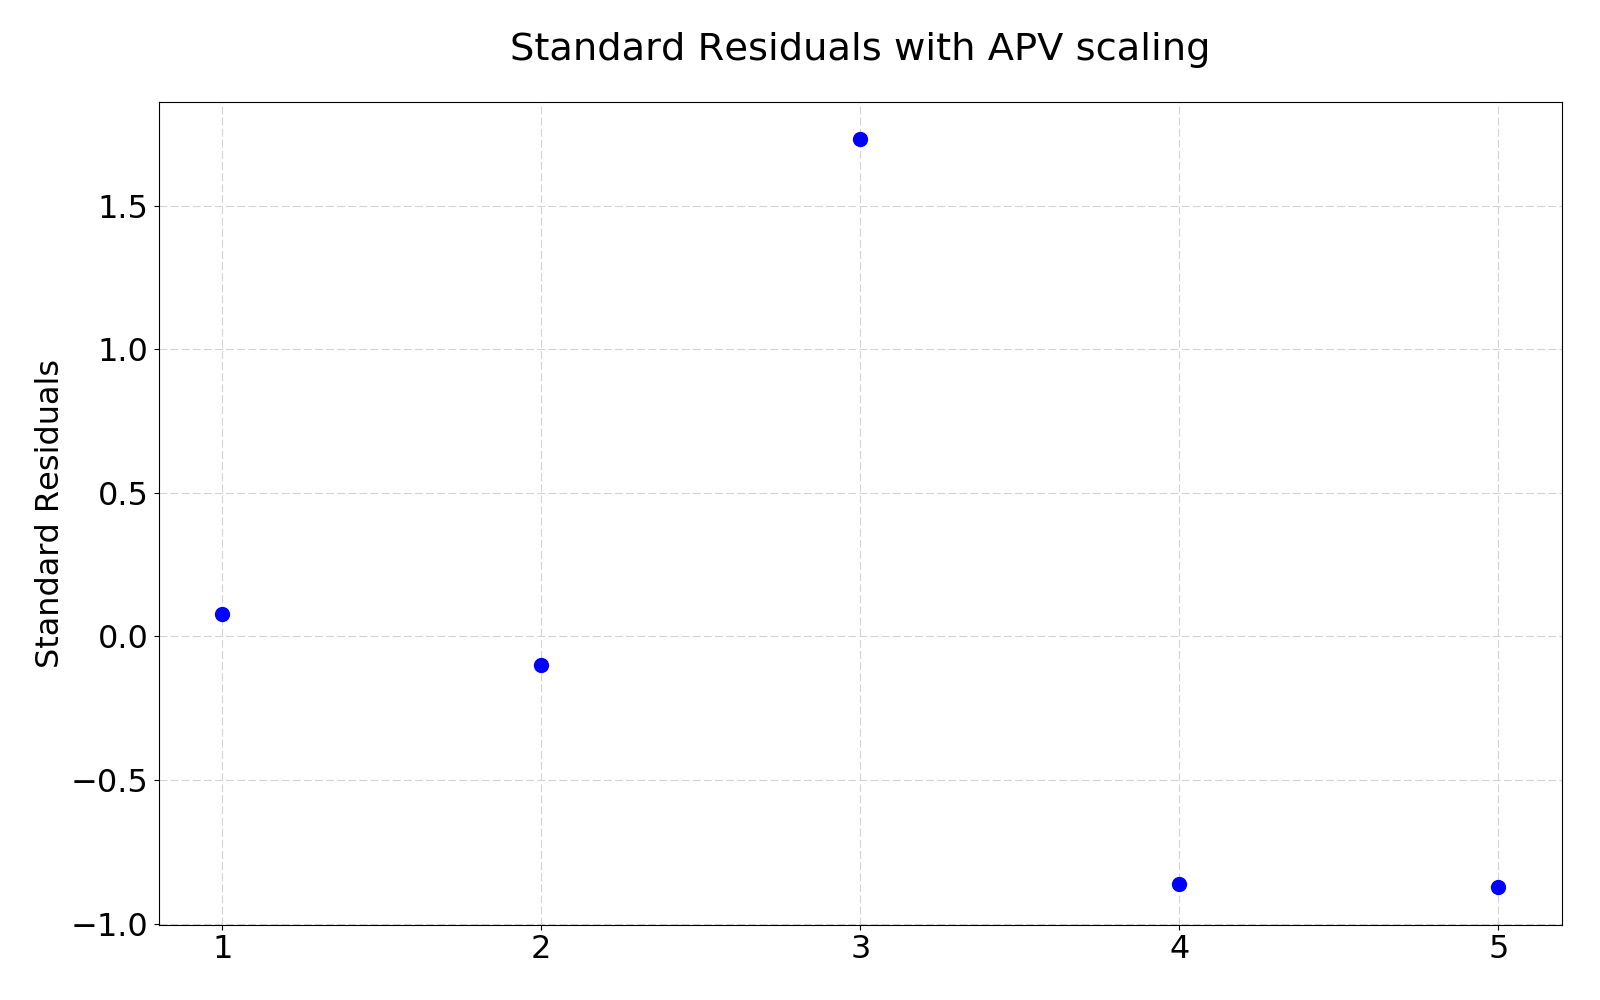
\includegraphics[trim = 0mm 0mm 0mm 0mm, clip, width=1.0\textwidth]{figures/ReliabilityExample/v55/StandardResidualsWithAPV.png}
	\caption{Ranging example - adding additional observations - standard residuals}
    \label{Fig:Ex1AddedObsStdRes}
\end{figure}

\subsection{Angles Example}

An analogous example to the ranges-only example involves only azimuth angle observations, as shown in figure \ref{Fig:Ex2Map}. As in the previous example, the position of interest is located at [0,10], measurement noise of 0.1$^{\circ}$ 1-$\sigma$ is employed, and the measurement uncertainty is also set as 0.1$^{\circ}$ 1-$\sigma$.

\newpage

\begin{figure}[!htb] 
    \centering
    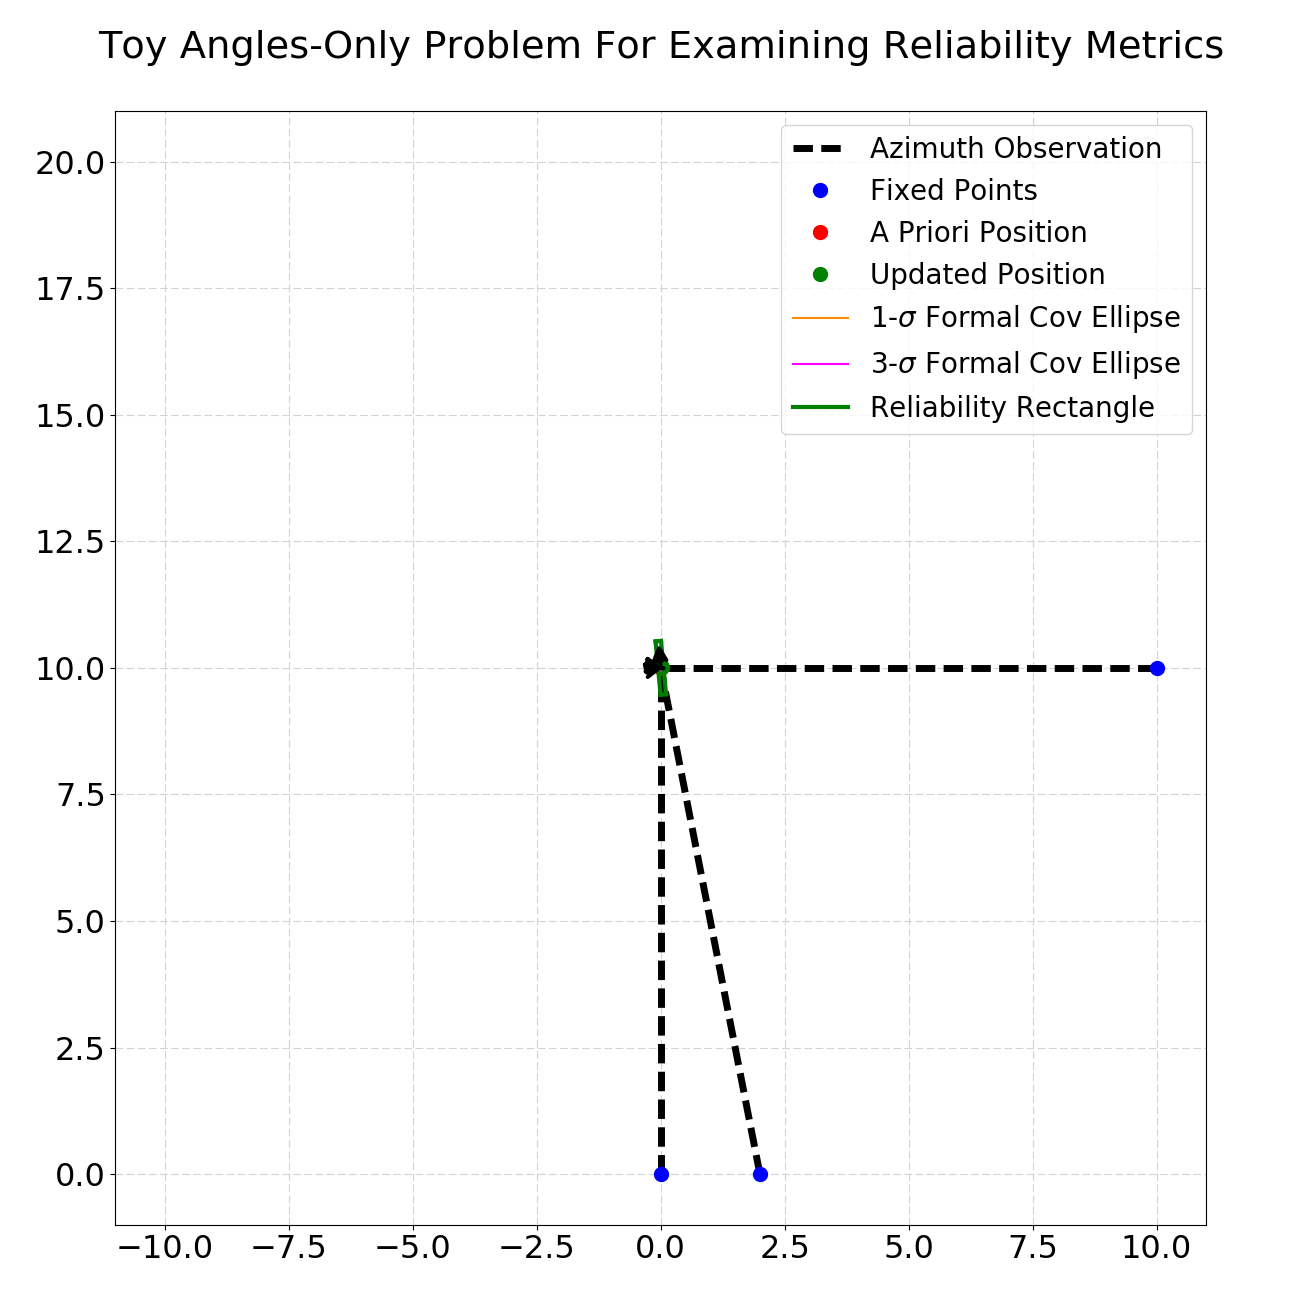
\includegraphics[trim = 0mm 0mm 0mm 5mm, clip, width=0.9\textwidth]{figures/ReliabilityExample/v22/Map.png}
    \caption{Angles example - map}
    \label{Fig:Ex2Map}
\end{figure}

\newpage

Figure \ref{Fig:Ex2MapZoom} provides a zoomed-in view of the region around the point of interest, with the formal uncertainty and reliability rectangle more visible. Unlike in Example 1, the reliability rectangle has large magnitude in the North-South axis due to lack of redundancy in that direction from having only one station to the East providing a direction observation.

\begin{figure}[!htb]
    \centering
    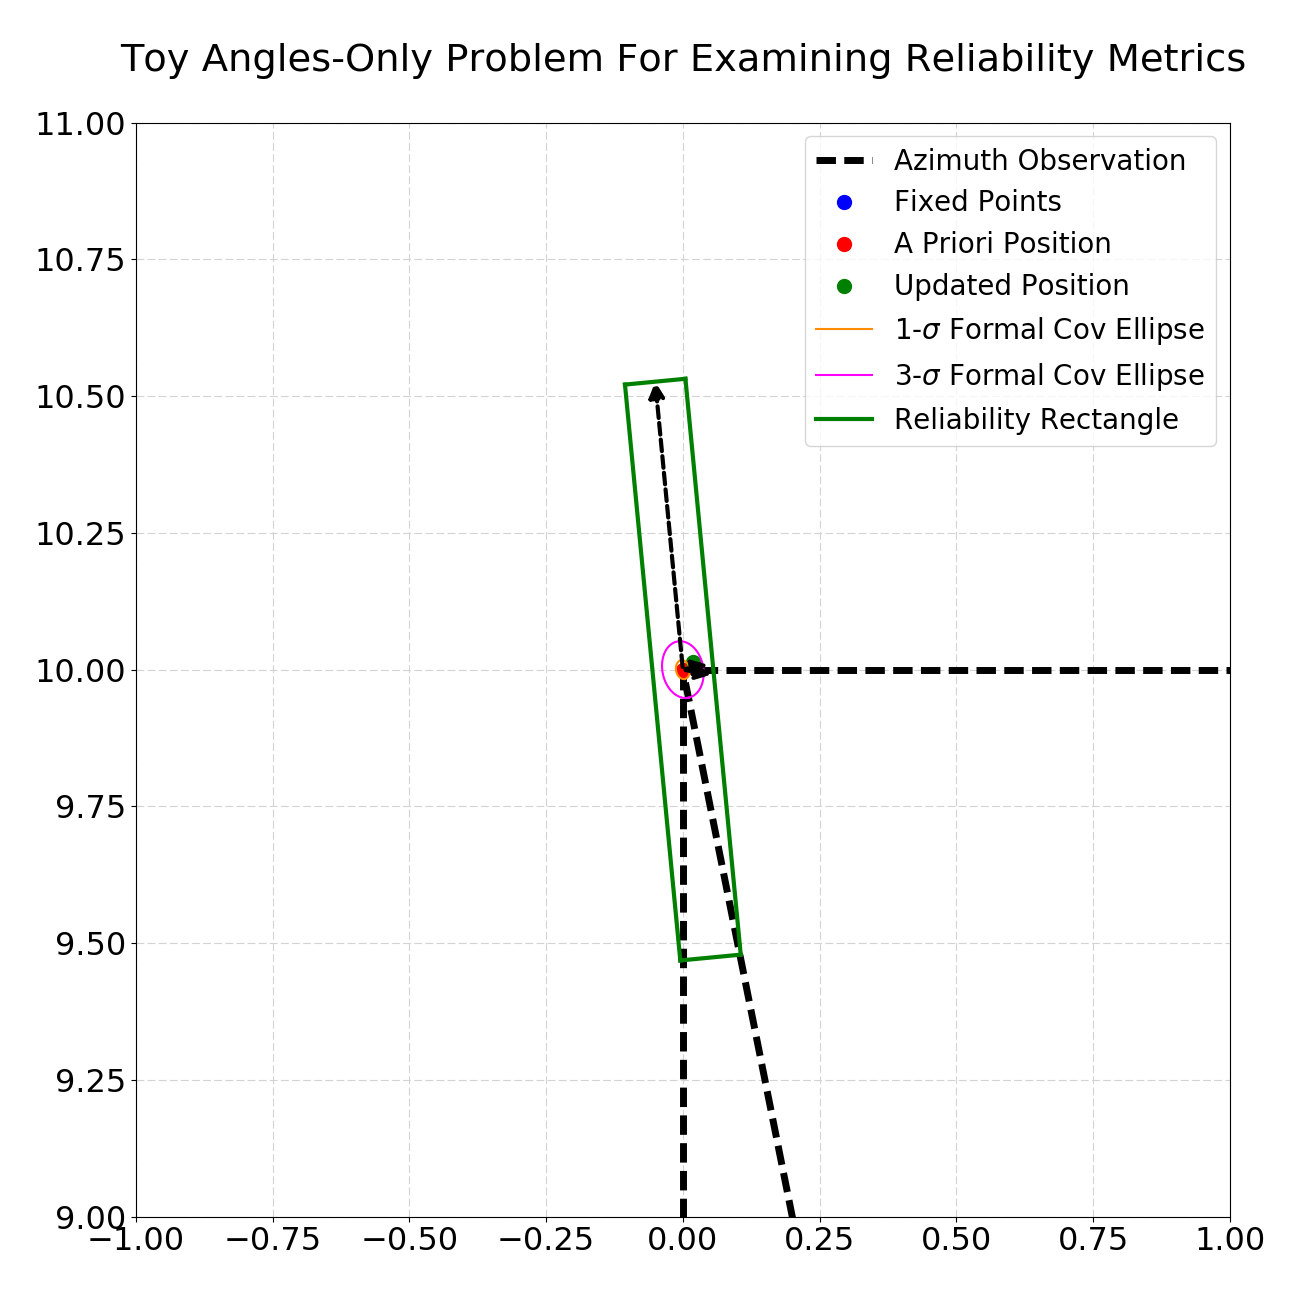
\includegraphics[trim = 0mm 0mm 0mm 5mm, clip, width=0.9\textwidth]{figures/ReliabilityExample/v22/MapZoomed.png}
    \caption{Angles example - zoomed map}
    \label{Fig:Ex2MapZoom}
\end{figure}

\newpage

The redundancy values (local reliability) for the three observations highlight how the third observation has almost no redundancy, as shown in figure \ref{Fig:Ex2redundancy}.

\begin{figure}[!htb]
    \centering
    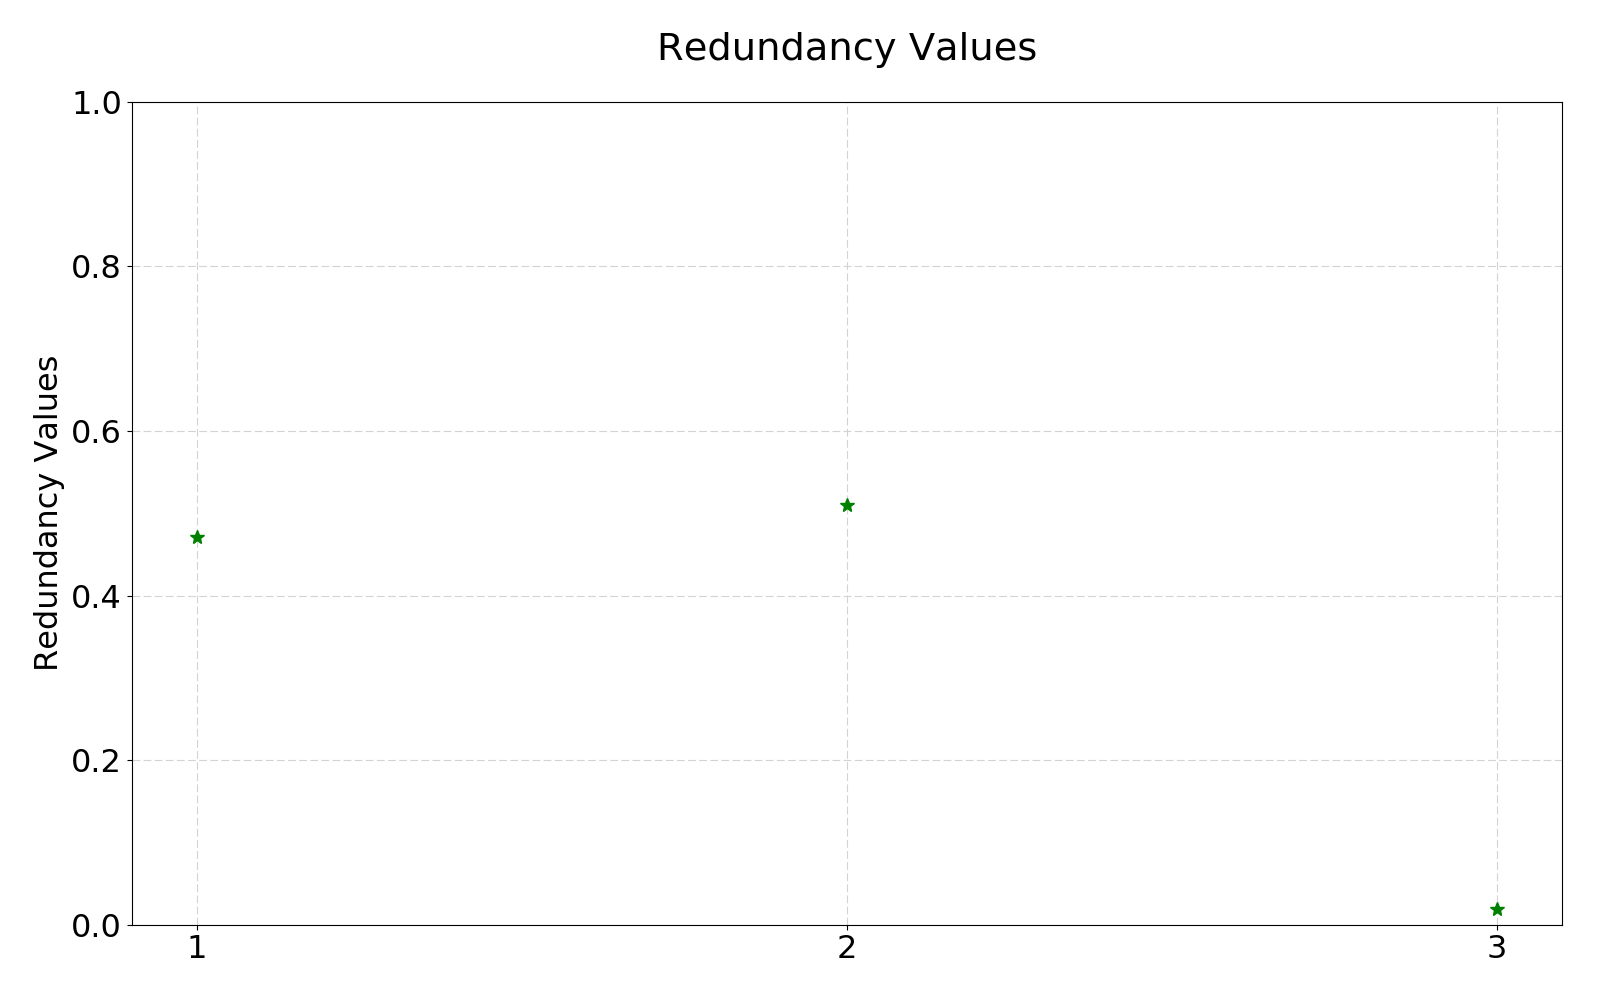
\includegraphics[trim = 0mm 0mm 0mm 0mm, clip, width=1.0\textwidth]{figures/ReliabilityExample/v22/Redundancy.png}
    \caption{Angles example - redundancy values}
    \label{Fig:Ex2redundancy}
\end{figure}

\newpage

The minimum detectable bias values (internal reliability) for the three observations, as shown in figure \ref{Fig:Ex2minDetBias}, reveals how the third observation has a significantly larger magnitude due to the poor redundancy of that observation:

\begin{figure}[!htb]
    \centering
    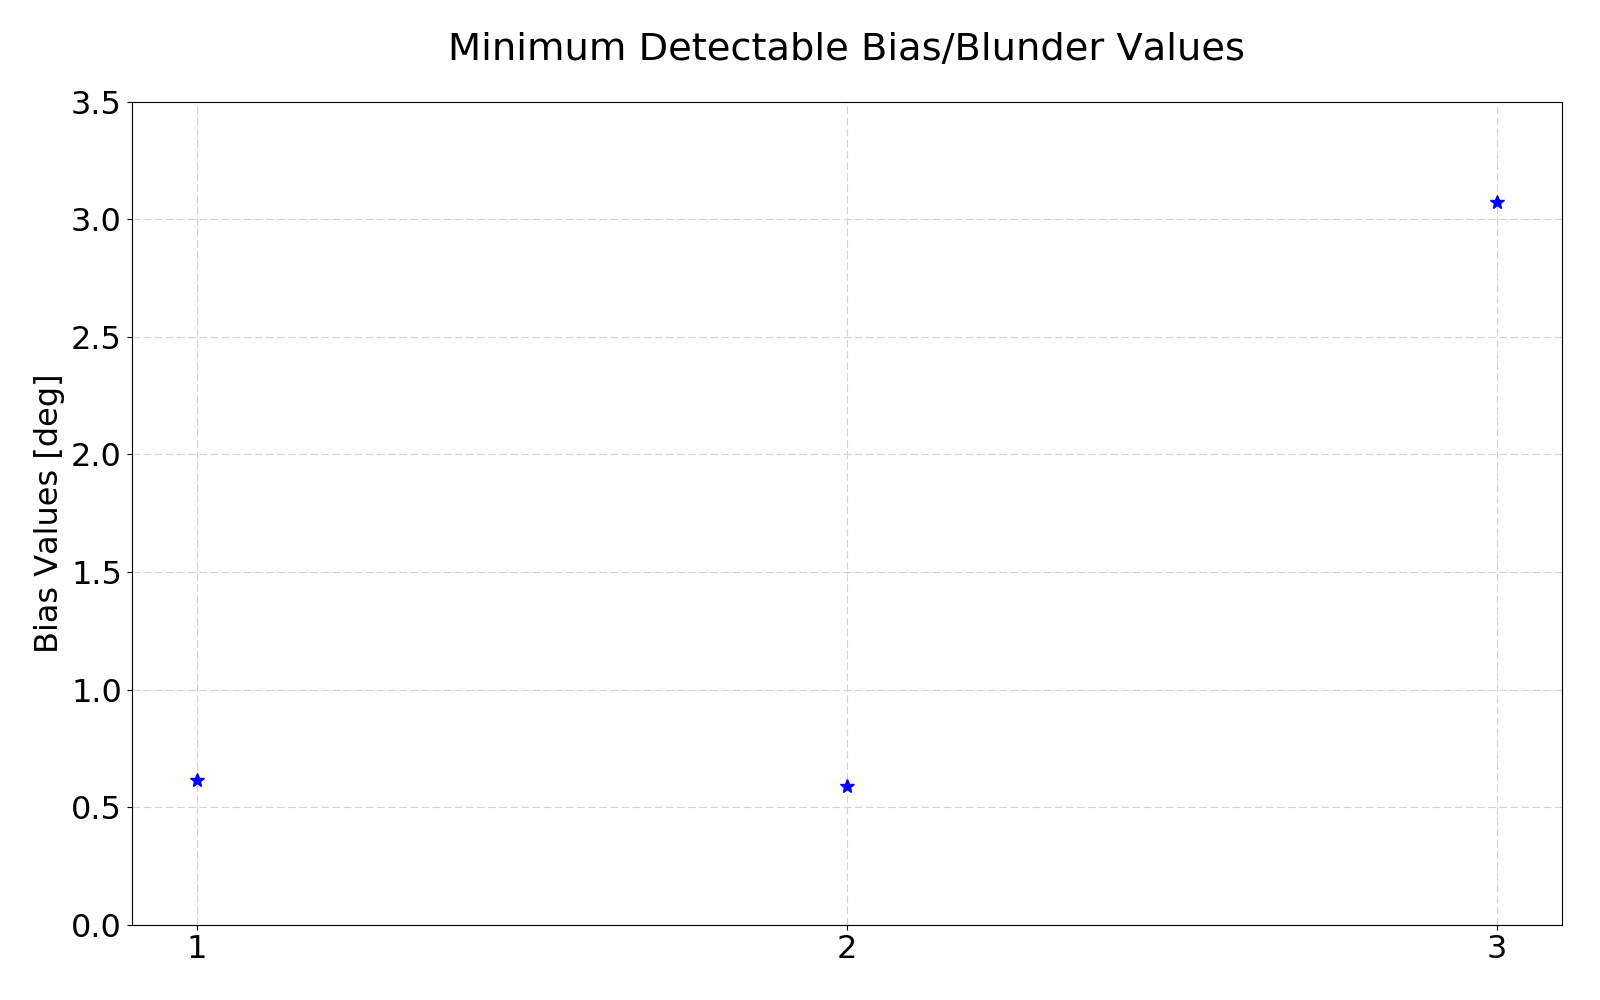
\includegraphics[trim = 0mm 0mm 0mm 0mm, clip, width=1.0\textwidth]{figures/ReliabilityExample/v22/MinDetBias.png}
    \caption{Angles example - minimum detectable bias values}
    \label{Fig:Ex2minDetBias}
\end{figure}

\newpage

The external reliability vector magnitudes for the three observations, as shown in figure \ref{Fig:Ex2ExtVectMag}, similarly shows the third observation has a much larger magnitude than the other two observations:

\begin{figure}[!htb]
    \centering
    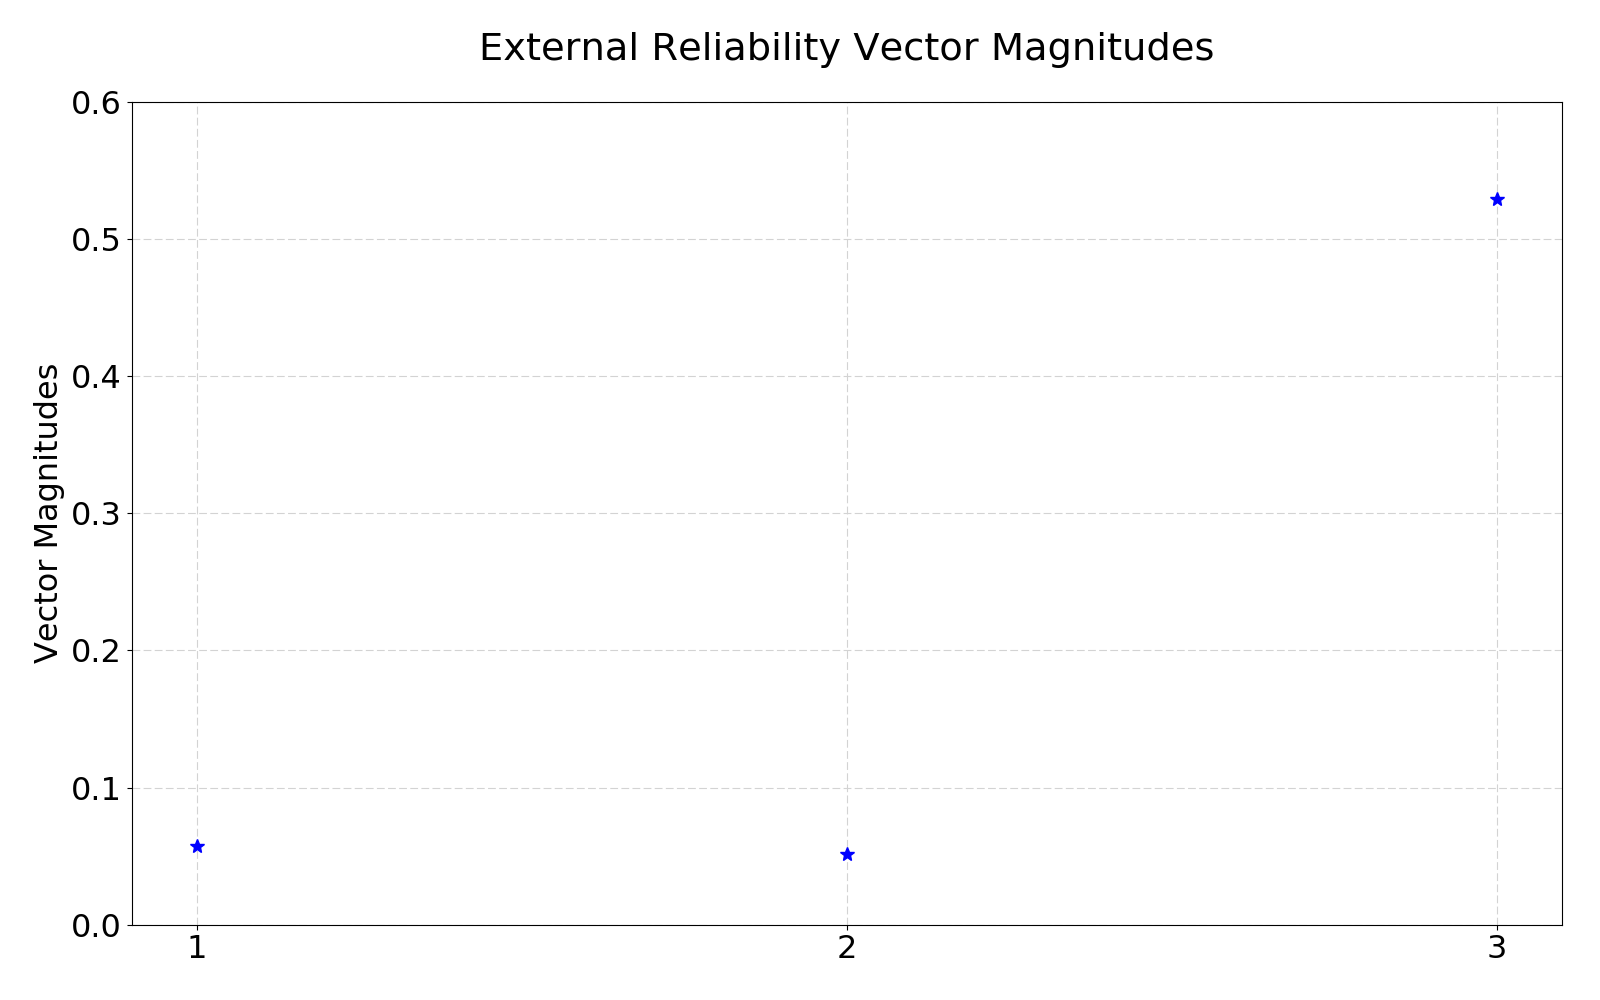
\includegraphics[trim = 0mm 0mm 0mm 0mm, clip, width=1.0\textwidth]{figures/ReliabilityExample/v22/ExtRelVectMags.png}
    \caption{Angles example - external reliability vector magnitudes}
    \label{Fig:Ex2ExtVectMag}
\end{figure}

\newpage

Just as in the ranges example above, the minimum detectable bias computed for the East station range observation is added to that observation, as shown in figure \ref{Fig:Ex2MapZoomBlunder}. The result: the estimated position now lies approximately on the northern edge of the reliability rectangle. (The estimated position lands exactly on the edge if no measurement noise is added.)

\begin{figure}[!htb]
    \centering
    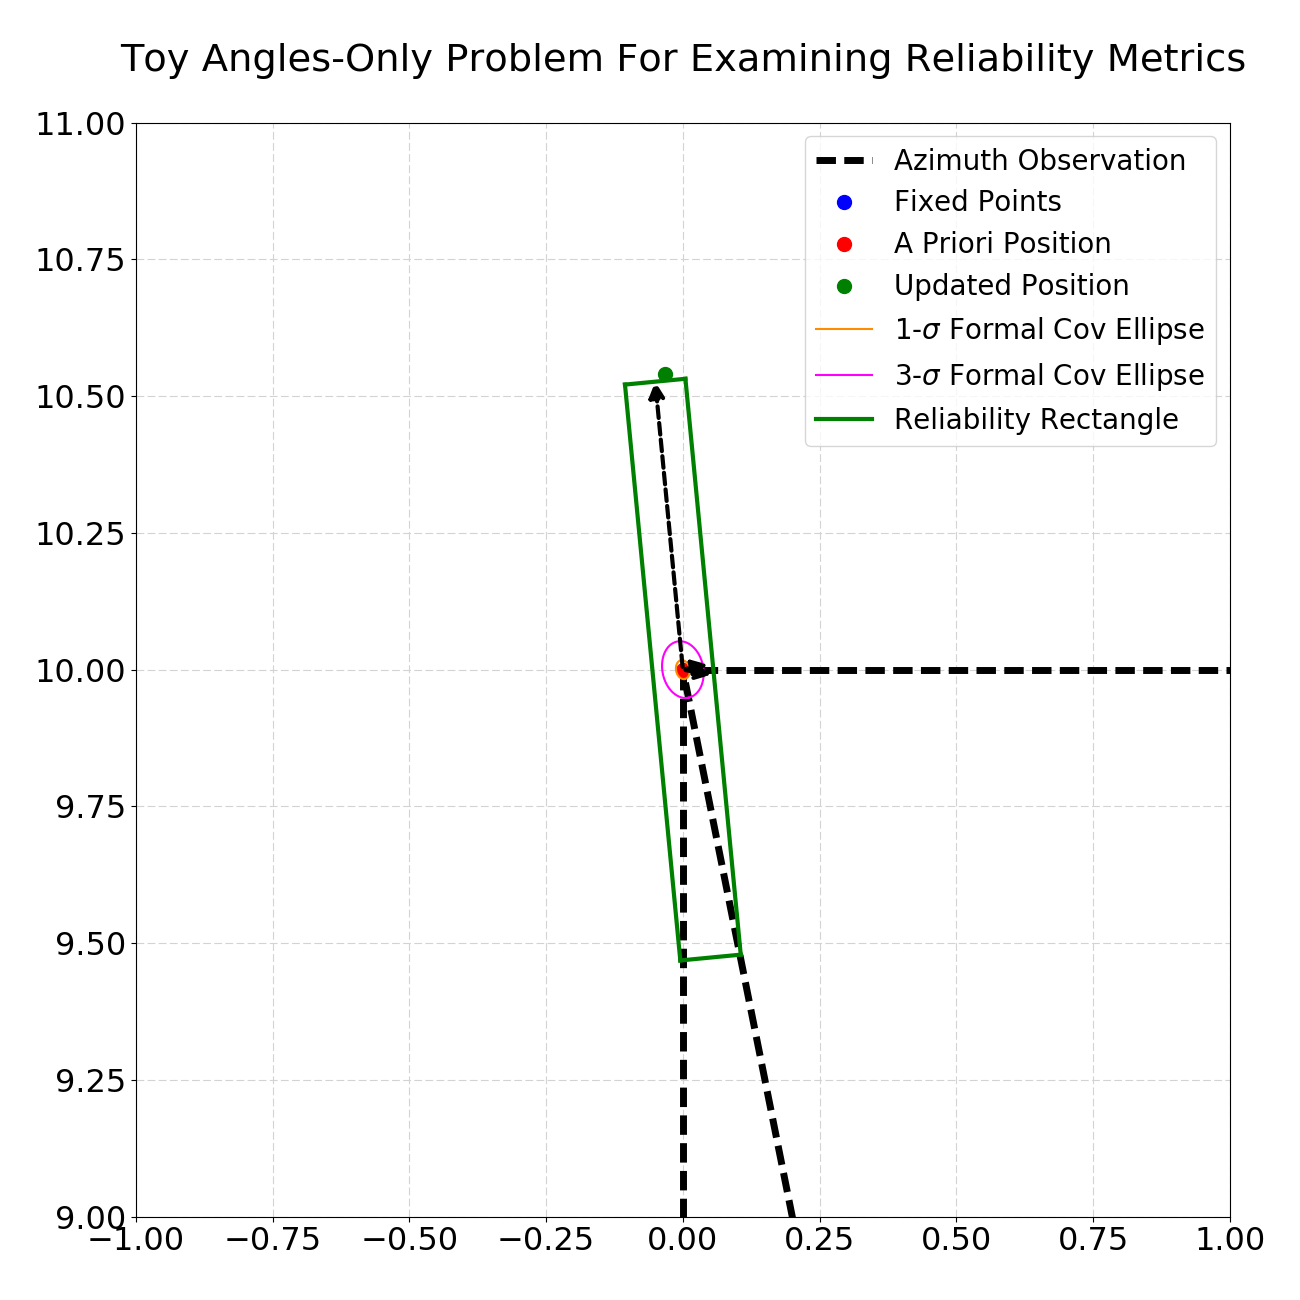
\includegraphics[trim = 0mm 0mm 0mm 5mm, clip, width=0.9\textwidth]{figures/ReliabilityExample/v26/MapZoomed.png}
    \caption{Angles example - east station blunder}
    \label{Fig:Ex2MapZoomBlunder}
\end{figure}

\newpage

Again just as in the ranges example above, the standard residuals do not reveal that the east station observation has a blunder, due to the lack of redundancy for that observation, as shown in figure \ref{Fig:Ex2StdRes}. 

\begin{figure}[!htb]
    \centering
    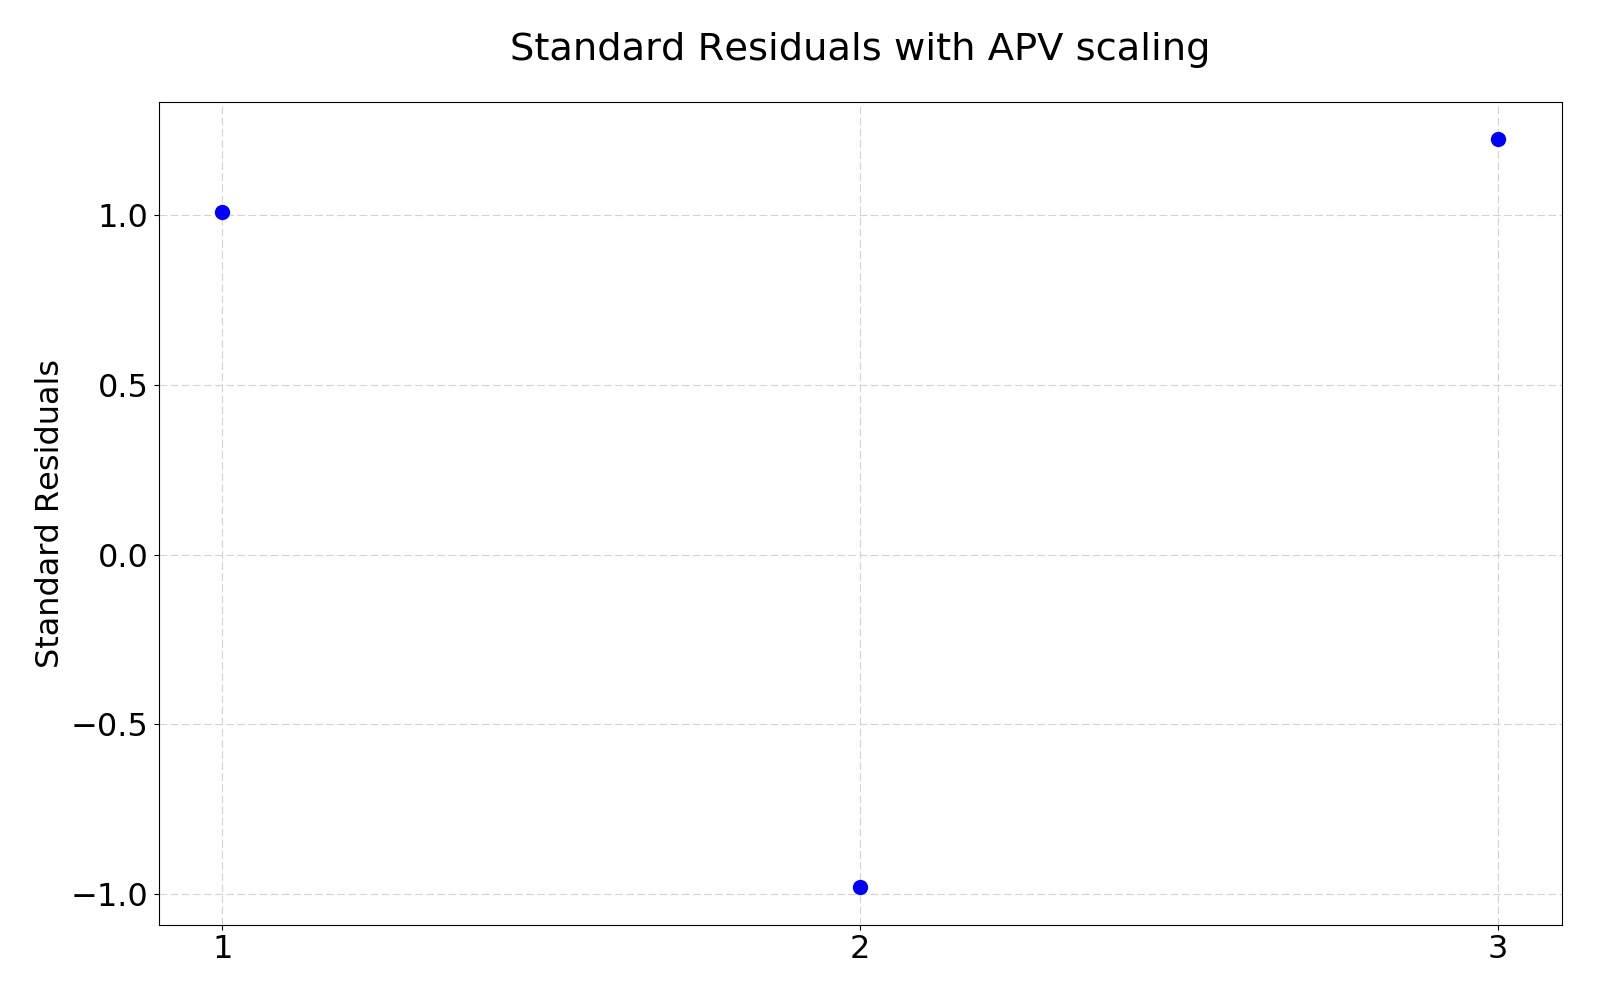
\includegraphics[trim = 0mm 0mm 0mm 0mm, clip, width=1.0\textwidth]{figures/ReliabilityExample/v56/StandardResidualsWithAPV.png}
    \caption{Angles example - standard residuals with east station blunder}
    \label{Fig:Ex2StdRes}
\end{figure}

\newpage

To address the lack of redundancy, another station can be added to the east, as shown in figure \ref{Fig:Ex2AddedObsMap}. 

\begin{figure}[!htb]
    \centering
    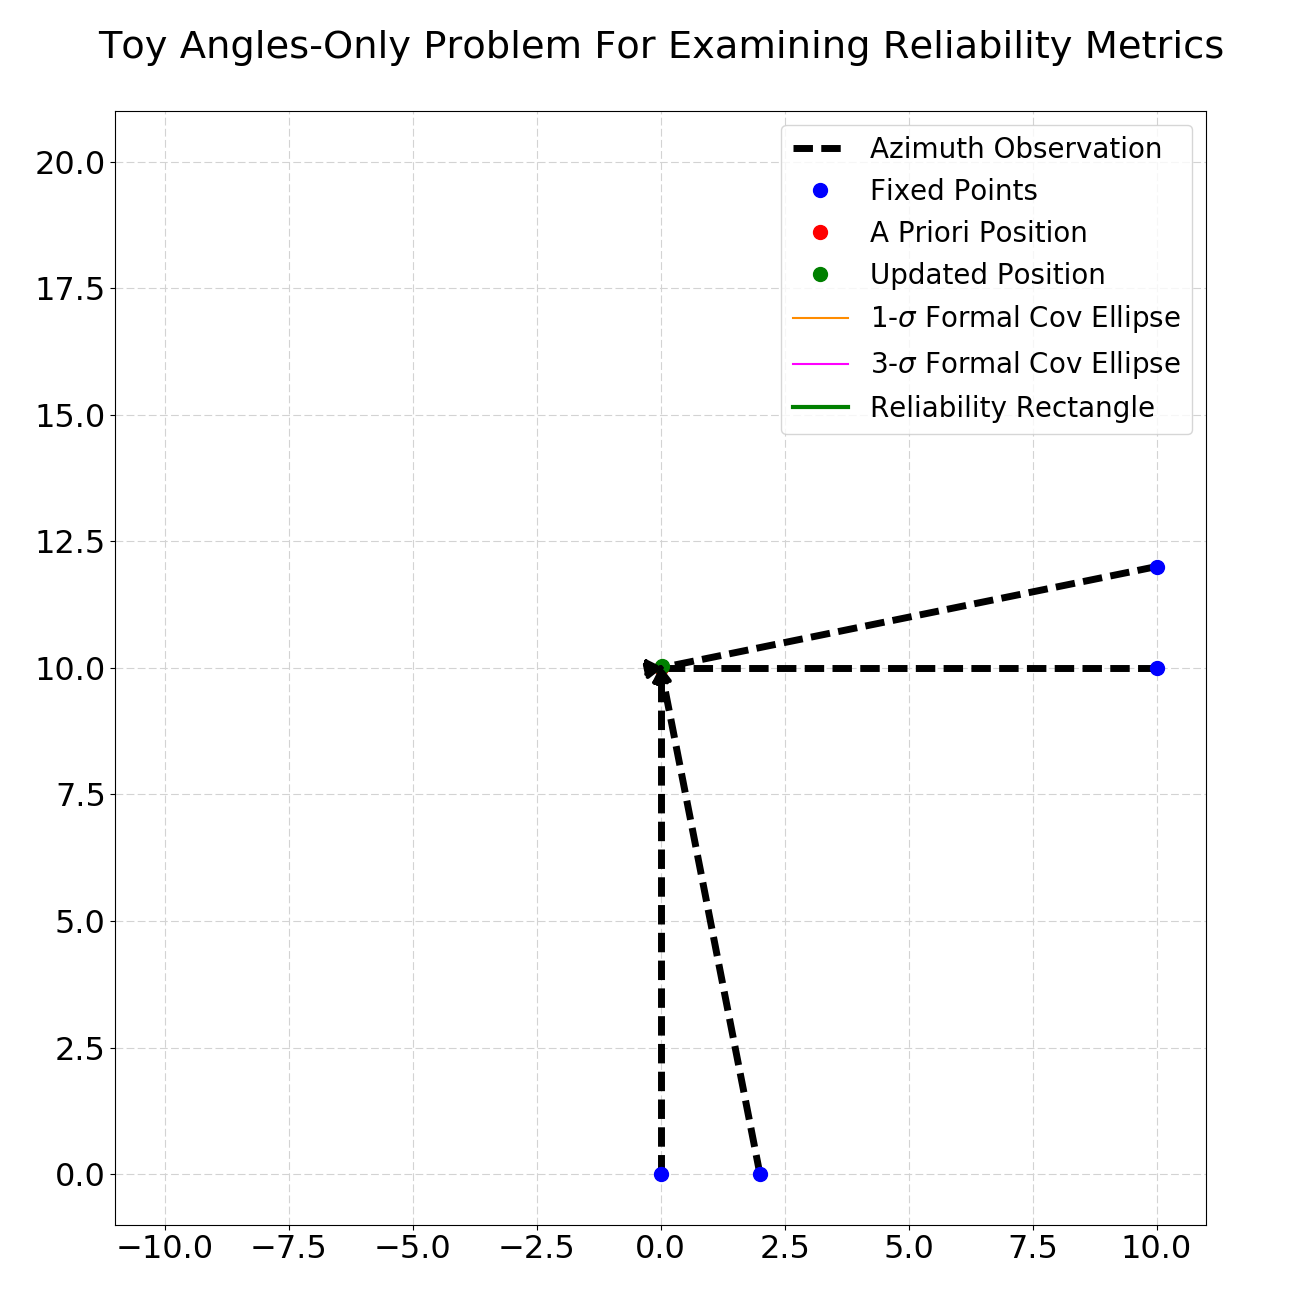
\includegraphics[trim = 0mm 0mm 0mm 5mm, clip, width=0.9\textwidth]{figures/ReliabilityExample/v24/Map.png}
    \caption{Angles example - adding additional observations}
    \label{Fig:Ex2AddedObsMap}
\end{figure}

\newpage

Zooming in on the estimated position reveals the impact of this additional observation on the reliability rectangle, as shown in figure \ref{Fig:Ex2AddedObsMapZoom}:

\begin{figure}[!htb]
    \centering
    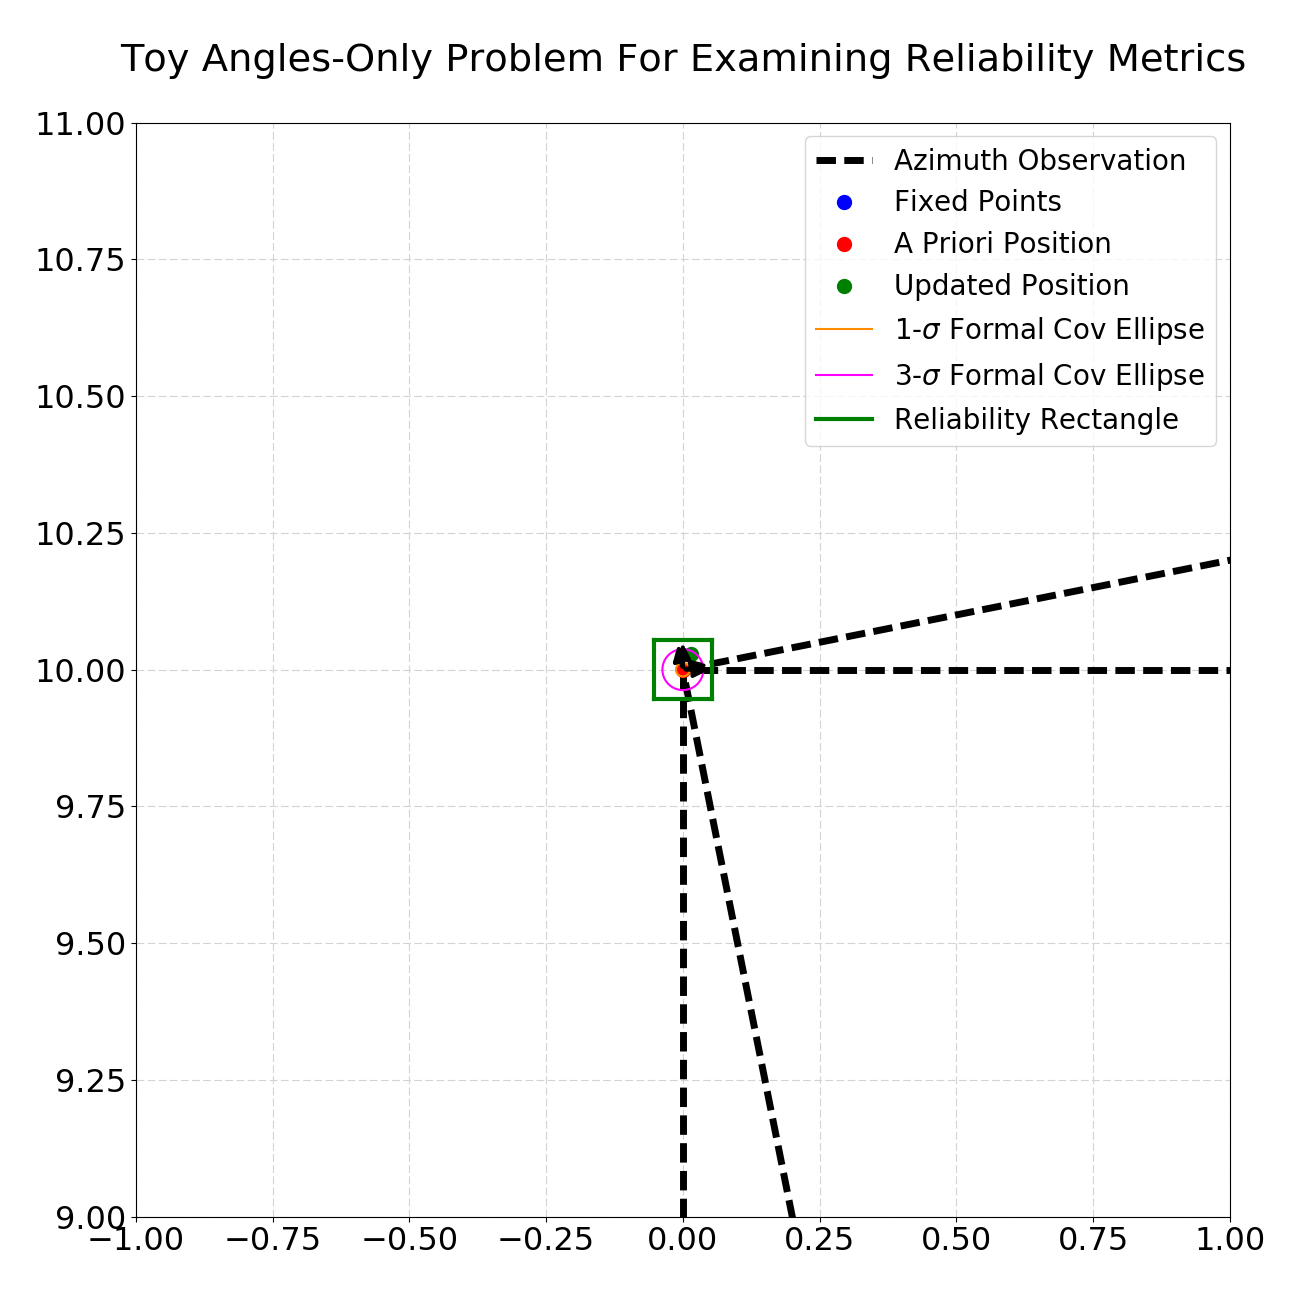
\includegraphics[trim = 0mm 0mm 0mm 5mm, clip, width=0.9\textwidth]{figures/ReliabilityExample/v24/MapZoomed.png}
    \caption{Angles example - adding additional observations}
    \label{Fig:Ex2AddedObsMapZoom}
\end{figure}

\newpage

\section{User Actions}

After an adjustment is processed, the surveyor should first verify that all observations have sufficient redundancy and no estimated points have unacceptably large reliability rectangles. Without good redundancy and reliability for each observation, metrics like standard residuals are not reliable indicators of potential blunders in the system.

Once good redundancy and reliability of all observations has been established, the standard residuals can be evaluated. If the standard residual test metric magnitude computed in equation \ref{eq:TestMetricStdRes} for a particular observation exceeds the threshold computed in equation \ref{eq:InvCDF}, the standard residual value is displayed as red text in the Measurement Residuals table. 

The user may wish to check each of these marked observations for blunders, with a focus on the data and/or sites involved in that measurement. Note that one blunder can affect many other quantities in the adjustment (estimated states and post-fit residuals). Thus the user is strongly encouraged to look for and correct only one blunder at a time, starting with the observation that has the largest standard residual test metric. After fixing that largest blunder, the user should re-run the adjustment and determine via the standard residuals (and other metrics such as the Chi-Squared Test) if more investigation is needed. Note that if the method of ``fixing'' the largest blunder results in poor redundancy/reliability, see above - the standard residuals may not be reliable anymore.

An important note: due to how the standard residual threshold is computed in equation \ref{eq:InvCDF}, if the redundancy value for an observation is low, the threshold value can become quite large. As a result, an observation with a large standard residual and low redundancy can still pass the hypothesis test and not be marked as red. Yet another reason it is vital to ensure all observations have reasonable redundancy. If the user encounters such an observation, we recommend the user collect more observations as needed to address the lack of redundancy in the survey itself if at all possible. If it is not possible, we recommend still investigating the largest residuals, even if they are not marked as failed the hypothesis test.

The user may also encounter smaller standard residuals that fail the hypothesis test and thus are marked as red. These observations likely have strong redundancy and small prescribed measurement uncertainty, and thus the relatively small raw residual is still large enough to fail the standard residuals hypothesis test. GPS vector observations often fall into this category, because GPS vector uncertainties are notoriously optimistic. Thus the user can likely ignore these relatively small standard residuals without significant impact on the final adjustment solution. If the user is feeling ambitious though, he or she can increase the prescribed uncertainty for that observation type, likely making that uncertainty more realistic and changing the standard residuals hypothesis test to passing.

One final note: the user should also keep an eye on the Chi-Squared global fit test to determine if there are any blunders remaining in the observations. If in the unlikely event there are large standard residuals but due to low redundancy values none of those residual fail the hypothesis test, it is like the Chi-Squared test will still fail.
